\documentclass[11pt,letterpaper]{article}

% Essential packages
\usepackage[utf8]{inputenc}
\usepackage[T1]{fontenc}
\usepackage[margin=1in]{geometry}
\usepackage{fancyhdr}
\usepackage{graphicx}
\usepackage{float}

% Math packages
\usepackage{amsmath}
\usepackage{amsfonts}
\usepackage{amssymb}
\usepackage{amsthm}

% Table packages
\usepackage{booktabs}
\usepackage{array}
\usepackage{tabularx}
\usepackage{longtable}

% List packages
\usepackage{enumitem}
\usepackage{float}

% Graphics and plotting
\usepackage{tikz}
\usepackage{pgfplots}
\pgfplotsset{compat=1.18}
\usepackage{subcaption}

% Citation and references
\usepackage[round,authoryear]{natbib}
\usepackage{url}

% Code listings and algorithms
\usepackage{listings}
\usepackage{xcolor}
\usepackage{algorithm}
\usepackage[noend]{algpseudocode}

% Configure code listings for Python
\lstset{
    language=Python,
    basicstyle=\ttfamily\small,
    keywordstyle=\color{blue},
    commentstyle=\color{gray},
    stringstyle=\color{red},
    showstringspaces=false,
    breaklines=true,
    frame=single,
    numbers=left,
    numberstyle=\tiny\color{gray},
    captionpos=b
}

% Hyperlinks (load last)
\usepackage[colorlinks=true,linkcolor=blue,citecolor=blue,urlcolor=blue]{hyperref}

% Custom commands for common actuarial notation
\newcommand{\E}{\mathbb{E}}
\newcommand{\Var}{\text{Var}}
\newcommand{\Cov}{\text{Cov}}
\newcommand{\Prob}{\mathbb{P}}

% Header and footer setup
\pagestyle{fancy}
\fancyhf{}
\fancyhead[L]{Ergodicity Simulation Framework for Insurance}
\fancyhead[R]{}
\fancyfoot[C]{\thepage}

% Title page information
\title{\Large \textbf{Ergodicity Economics in Property \& Casualty Insurance: \\
A Simulation Framework for Understanding Risk Appetite}}

\author{Alex Filiakov, ACAS\\
\texttt{alexfiliakov@gmail.com}}

\date{\today}

\begin{document}

\maketitle

\begin{abstract}
Guaranteed cost insurance programs often destroy shareholder value, yet companies continue buying them. Or they blindly match peer deductibles without understanding the true economics of their programs. This paper introduces the first open-source simulation framework for time-average optimization of corporate risk transfer, challenging conventional wisdom that treats insurance as a cost to minimize. Using ergodicity economics principles and 100,000 Monte Carlo paths over 50-year horizons, we demonstrate that optimal strategies emerge from maximizing time-average growth rates rather than minimizing expected costs.

The framework models complete corporate balance sheet dynamics under realistic loss distributions, revealing that moderate retention strategies consistently dominate both guaranteed cost and self-insurance extremes. Small companies rationally pay substantial premium loadings over actuarially fair rates because insurance alters multiplicative wealth dynamics in ways invisible to ensemble-average analysis. Capitalization level, operating margins, and asset turnover drive optimal deductible selection far more than industry benchmarks or peer conventions.

This simulation-based framework provides tools for company-specific risk transfer optimization, empowering CFOs, risk managers, and actuaries to move beyond conventional expected value analysis toward rigorous, growth-focused insurance purchasing decisions.
\\\\
\textbf{Keywords:} ergodicity economics, insurance purchasing, corporate risk management, time-average growth, deductible optimization, Monte Carlo simulation, multiplicative dynamics, risk modeling, property \& casualty insurance, Kelly Criterion, balance sheet modeling, retention strategy
\end{abstract}

\newpage
\tableofcontents
\newpage

\section{Executive Summary}

\subsection{The Challenge}

Corporate insurance purchasing decisions typically rely on peer benchmarking, broker recommendations, or rules of thumb that may bear little relation to a company's specific financial circumstances. When evaluating whether to select a \$100K or \$500K deductible, most organizations lack rigorous analytical frameworks to quantify how different retention strategies affect long-term shareholder value. Traditional cost-benefit analysis focuses on minimizing expected costs, but this approach systematically undervalues insurance for companies where balance sheet dynamics and growth trajectories depend critically on avoiding capital impairment.

The fundamental question facing corporate decision-makers is not "What deductible do similar companies choose?" but rather "What retention strategy maximizes our long-term growth given our specific capitalization, operating margins, and loss exposures?" Answering this question requires moving beyond expected value calculations to consider how insurance programs alter the time path of corporate wealth accumulation under uncertainty.

\subsection{A New Framework for Risk Transfer Optimization}

This paper introduces an open-source simulation framework that models complete corporate balance sheet dynamics under realistic loss distributions and insurance programs. Rather than treating insurance as a simple cost minimization problem, the framework optimizes time-average growth rates, the metric that determines actual shareholder value creation over multi-year horizons. Using rigorous Monte Carlo simulation with customizable paths and time periods, the model tracks how different deductible strategies affect equity accumulation, retained earnings, cash flow, and ultimately long-term enterprise value.

The framework accounts for critical financial realities often ignored in traditional analysis: losses compound through balance sheet effects, claim payments follow multi-year schedules requiring collateral, operating margins buffer loss impacts, and asset turnover determines exposure intensity. By modeling these dynamics explicitly, the simulation reveals optimization opportunities invisible to conventional expected value frameworks.

\subsection{Key Findings}

The analysis produces several insights relevant to corporate risk transfer decisions:

\vspace{\baselineskip}

\textbf{The Retention Sweet Spot.} Moderate retention strategies consistently outperform both extremes. Companies maximizing long-term growth typically select deductibles in the middle of the feasible range: neither guaranteed cost (zero deductible) nor complete self-insurance. This finding challenges the common practice of defaulting to guaranteed cost programs for "certainty" or aggressively high retentions to "save premium dollars." The optimal strategy balances premium costs against catastrophic loss protection, recognizing that both excessive coverage and insufficient protection leave value on the table.

\vspace{\baselineskip}

\textbf{Company Size Drives Strategy.} Capitalization level relative to potential loss severity matters far more than industry sector or revenue scale. A company with \$5M in equity derives fundamentally different insurance value than a \$25M company facing identical loss distributions. Smaller companies benefit substantially from insurance protection even at higher relative premium costs, while larger organizations can profitably retain more risk.

\vspace{\baselineskip}

\textbf{Premium Loadings and Rational Insurance.} Small to mid-market companies can rationally purchase insurance even when premiums substantially exceed expected losses. This finding contradicts traditional expected value logic, which views such programs as "too expensive." The framework demonstrates that insurance creates value by reducing the multiplicative impact of large losses on balance sheet growth, particularly for companies where individual catastrophic events would meaningfully erode equity. The relevant question is not whether premiums exceed expected claims but whether insurance enhances time-average growth rates net of all costs.

\vspace{\baselineskip}

\textbf{Operating and Financial Characteristics Matter.} Asset turnover ratios and operating margins interact with capitalization to determine optimal strategies. Capital-efficient companies generating high revenues relative to their balance sheet face more frequent loss exposures per dollar of equity, amplifying insurance value. Similarly, low-margin operations exhibit greater sensitivity to retention choices because premium costs and retained losses represent larger fractions of net income. These company-specific factors drive optimal deductible selection far more than industry conventions or broker guidelines. This operational-dependent relationship explains why peer benchmarking often produces suboptimal strategies: companies at different operational efficiencies require different risk transfer approaches.

\subsection{Practical Implications and Value Creation}

Organizations that optimize retention strategies based on their specific financial characteristics rather than peer benchmarking or conventional wisdom can potentially create substantial shareholder value. The framework provides tools to quantify this impact for individual companies, translating abstract insurance decisions into concrete projections of equity accumulation under different scenarios.

Current corporate insurance programs often exhibit one of two suboptimal patterns: excessive guaranteed cost coverage that trades growth for perceived certainty, or overly aggressive retention that exposes balance sheets to multiplicative erosion from tail losses. Both approaches leave value on the table. Companies implementing first-principles optimization can redirect these inefficiencies toward enhanced long-term growth.

The framework is particularly relevant for organizations experiencing significant changes in capitalization, business model, or risk profile; situations where historical practices or peer comparisons provide limited guidance. It enables systematic evaluation of insurance programs as capital allocation decisions rather than cost centers, shifting the conversation from "How do we minimize insurance spending?" to "What retention strategy maximizes enterprise value?"

\subsection{Implementation Path}

The simulation framework is open-source and available for implementation by corporate risk management teams working with actuarial professionals. Organizations interested in applying this approach to their specific circumstances should:

\begin{itemize}
    \item \textbf{Download the framework} and review the technical documentation, starting with this guide:

        \url{https://docs.mostlyoptimal.com/api/tutorials/01_getting_started.html}

    \item \textbf{Form an internal task force} including finance, risk management, and actuarial expertise to evaluate the methodology and identify company-specific calibration requirements
    \item \textbf{Calibrate loss distributions} using historical claims data, industry benchmarks, and company-specific exposure analysis rather than relying solely on insurer estimates
    \item \textbf{Run company-specific simulations} incorporating actual balance sheet parameters, operating margins, capital structure, and growth projections
    \item \textbf{Evaluate current insurance programs} against optimized retention strategies to identify value creation opportunities
\end{itemize}

Important caveats: The specific numerical results presented in this paper depend on modeled assumptions and loss distributions that do not reflect individual company circumstances. The framework provides directional guidance and analytical tools, not prescriptive formulas. Optimal strategies require company-specific calibration incorporating industry dynamics, regulatory constraints, and other factors not fully modeled in the baseline analysis. Organizations should view the framework as enabling rigorous internal analysis rather than offering one-size-fits-all recommendations.

\subsection{Methodological Foundation}

The simulation framework models corporate balance sheet evolution under stochastic loss processes, tracking assets, liabilities, equity, revenues, operating income, insurance premiums, claim payments, collateral requirements, and retained earnings through annual or monthly time steps. Loss distributions incorporate three tiers (attritional, large, and catastrophic events) calibrated to realistic manufacturing company exposures. Insurance programs feature varying deductible and limit levels with premiums scaled to exposure base and loaded for insurer expenses. The model maintains complete accounting relationships and implements realistic claim payment schedules requiring multi-year collateral posting.

Time-average growth rate optimization provides the analytical lens, recognizing that companies experience temporal sequences of outcomes rather than statistical ensemble averages. This approach reveals insurance value that remains invisible when evaluating programs solely through expected cost minimization one year at a time. The framework is transparent and open-source, enabling peer review and adaptation to industry-specific requirements.

The analysis demonstrates that rigorous, company-specific optimization of corporate risk transfer programs is both feasible and valuable. Organizations willing to move beyond conventional practices toward first-principles evaluation can enhance long-term shareholder value while maintaining appropriate protection against catastrophic losses.

\section{Introduction}

When a \$10M company selects a \$100K deductible for its property and casualty insurance program, is that decision based on rigorous analysis or industry convention? When a CFO approves premiums that exceed expected losses by 50\%, is that rational or wasteful? These questions matter: as the global insurance market reaches \$10T annually, most companies lack analytical frameworks to optimize retention strategies or quantify insurance value beyond vague notions of "risk transfer" and "protection."

This paper develops a new simulation framework for analyzing \emph{corporate insurance purchasing decisions} through the lens of ergodicity economics. Unlike traditional expected value analysis, which treats insurance as a cost to be minimized and appeals to psychological utility curves to justify risk aversion, our approach recognizes that insurance fundamentally alters the \emph{time-average growth rate} of companies facing multiplicative risks. We demonstrate that this shift in perspective reveals substantial insurance value invisible to conventional analysis and produces counterintuitive results that challenge standard industry practices.

\subsection{The Problem with Expected Value Analysis}

Traditional approaches to corporate insurance decisions rely on ensemble averages and expected value calculations. Under this framework, insurance appears economically irrational whenever premiums exceed expected losses: why pay \$150K annually to cover losses averaging \$100K? The standard answer invokes risk aversion, behavioral biases, or non-economic factors like regulatory requirements and stakeholder preferences.

But this framing misses something fundamental. Real companies don't experience ensemble averages, they experience \emph{temporal sequences of outcomes} that compound multiplicatively over time. A company suffering a \$5M uninsured loss doesn't care that the ensemble average across thousands of parallel universes would have been \$2M. What matters is the actual path its balance sheet follows: equity eroded, credit constrained, growth opportunities foreclosed.

Traditional expected value analysis faces several critical limitations when applied to corporate insurance decisions:
\begin{itemize}
    \item \textbf{Ignores path dependence:} Losses compound through balance sheet effects, making the \emph{sequence} of outcomes as important as their statistical distribution
    \item \textbf{Misses multiplicative dynamics:} Wealth evolves through percentage changes that compound, not additive changes that average
    \item \textbf{Overlooks company-specific factors:} Optimal strategies depend on capitalization, margins, and exposure intensity, not on industry benchmarks
    \item \textbf{Encourages peer benchmarking:} "What deductible do similar companies choose?" often substitutes for first-principles analysis, potentially creating systemic antipatterns
\end{itemize}

These limitations matter most for growth-focused companies, where the question isn't "How do we minimize costs?" but rather "How do we maximize long-term shareholder value under uncertainty?"

\subsection{The Ergodicity Economics Approach}

Ergodicity economics, pioneered by \citet{peters2019ergodicity} and building on \citet{kelly1956new}, offers a fundamentally different lens for decision-making under uncertainty. The key insight: distinguish between \emph{ensemble averages} (expectations across many parallel scenarios) and \emph{time averages} (what individual entities experience over their actual lifetime). When these diverge, as they do for any system with multiplicative wealth dynamics and absorbing barriers like bankruptcy, optimizing ensemble averages leads to systematically poor long-term outcomes.

The Kelly Criterion, developed for gambling and investment allocation, provides the mathematical foundation: maximize the expected logarithm of wealth rather than expected wealth itself. This seemingly subtle shift from $\mathbb{E}[W]$ to $\mathbb{E}[\ln W]$ produces dramatically different optimal strategies because the logarithm penalizes downside outcomes multiplicatively. Applied to insurance, this framework reveals that variance reduction can enhance growth even when premiums substantially exceed actuarially fair rates. Precisely the situation corporate buyers face in competitive insurance markets.

\subsection{What This Paper Demonstrates}

We develop a comprehensive simulation framework that models corporate balance sheet dynamics under realistic loss distributions, insurance programs, and financial accounting relationships. The model tracks 100,000 Monte Carlo paths over 50-year horizons, computing time-average growth rates for companies across different capitalization levels, operating margins, asset turnover ratios, and insurance strategies.

The analysis produces several counterintuitive findings that challenge conventional wisdom:

\begin{itemize}
    \item \textbf{Guaranteed cost programs often destroy value.} Full coverage with zero deductible consistently underperforms moderate retention strategies, even though it eliminates all retained loss volatility. For larger companies, guaranteed cost can even underperform \emph{complete self-insurance}.

    \item \textbf{Moderate retention strategies dominate both extremes.} The optimal deductible typically falls in the middle of the feasible range—neither guaranteed cost nor self-insurance maximizes growth. This "retention sweet spot" emerges from balancing premium costs against catastrophic loss protection.

    \item \textbf{Capitalization is the dominant driver.} Company size relative to potential loss severity matters far more than industry sector, revenue scale, or absolute premium dollars. A \$5M company derives fundamentally different insurance value than a \$25M company facing identical loss distributions.

    \item \textbf{Asset turnover amplifies insurance value.} Capital-efficient companies generating high revenues relative to their balance sheet face disproportionately greater insurance value because they experience more frequent loss exposures per dollar of equity.
\end{itemize}

These findings emerge naturally from the ergodic framework but remain invisible to traditional expected value analysis. They suggest that many corporate insurance programs are suboptimally structured, leaving substantial value on the table through either excessive coverage (guaranteed cost) or insufficient protection (overly aggressive retention).

\subsection{A Framework, Not a Formula}

This paper provides a \emph{simulation framework} for studying time-average performance of insurance programs under flexible corporate dynamics, not a prescriptive formula for optimal deductibles. The specific numerical results depend heavily on loss distribution parameters, financial assumptions, and modeling choices, none of which perfectly reflect any particular company's reality.

The goal is not to recommend "all \$10M companies should buy \$250K deductibles" but rather to demonstrate \emph{how} ergodic analysis changes insurance valuation and to provide tools for company-specific optimization. We develop a rigorous mathematical foundation with 100,000-path Monte Carlo simulations, a fully specified corporate balance sheet model, and actuarially realistic loss distributions, and then use this machinery to explore the parameter space systematically.

The primary contribution is methodological: showing \emph{that} time-average growth optimization can be implemented for corporate insurance decisions, \emph{how} it produces qualitatively different recommendations than expected value analysis, and \emph{why} these differences matter for long-term shareholder value. Practitioners can adapt the framework to their specific circumstances, calibrating loss distributions to company data and incorporating constraints invisible to the baseline model.

\subsection{Implications}

The simulation results suggest that corporate insurance markets may be systematically mispricing insurance value. More precisely, \emph{correctly} pricing expected losses while \emph{undervaluing} the time-average growth benefits for certain buyer segments. Companies with low capitalization relative to potential losses should be willing to pay substantial premiums over actuarially fair rates, yet many pursue aggressive retention strategies driven by expected value logic or peer benchmarking.

We encourage corporate risk practitioners to:
\begin{itemize}
    \item \textbf{Study company-specific loss costs} using historical claims data, industry benchmarks, and exposure analysis rather than relying solely on insurer-provided estimates
    \item \textbf{Model corporate balance sheet dynamics} under stochastic loss scenarios to quantify growth impacts beyond point estimates of expected losses
    \item \textbf{Challenge guaranteed cost conventions} that may persist due to institutional inertia rather than economic optimization
    \item \textbf{Request time-average analytics} from insurance brokers and actuarial consultants, pushing the industry toward ergodic frameworks
\end{itemize}

Insurance should not be viewed merely as a cost center subject to minimization but as a \emph{strategic capital allocation decision} that fundamentally affects long-term growth trajectories. The simulation framework developed here provides the analytical foundation for making such decisions rigorously rather than conventionally.

\section{Theoretical Foundation}

\subsection{Ergodicity vs. Non-Ergodicity in Financial Systems}

The distinction between time averages and ensemble averages lies at the heart of ergodic economics, a framework pioneered by \citet{peters2019ergodicity} that challenges fundamental assumptions in economic theory. A stochastic process is ergodic if its time average equals its ensemble average:

\begin{equation}
\lim_{T \to \infty} \frac{1}{T} \int_0^T f(X_t) dt = \E[f(X)]
\end{equation}

For ergodic systems, what happens to an individual over time matches the average across many individuals at a single point in time. However, most economic processes violate this equality, creating a fundamental divergence between individual experience and statistical expectations.

The ensemble average represents the expected value across many parallel scenarios:
\begin{equation}
\langle W \rangle = \E[W_t] = \frac{1}{N} \sum_{i=1}^{N} W_i(t)
\end{equation}

where $W_i(t)$ represents the wealth of entity $i$ at time $t$. This is the traditional expected value used in most economic and actuarial analysis.

In contrast, the time average captures what a single entity experiences over its lifetime:
\begin{equation}
g_{\text{time}} = \lim_{T \to \infty} \frac{1}{T} \ln\left(\frac{W_T}{W_0}\right)
\end{equation}

For multiplicative processes with uncertainty, Jensen's inequality ensures these two averages diverge systematically, with profound implications for insurance and risk management \citep{peters2016evaluating}. Jensen's inequality states that for a random variable $W$ and a convex function $f$:

\begin{equation}
f(\E[W]) \leq \E[f(W)]
\end{equation}

In the context of multiplicative wealth dynamics, this means that the expected growth rate (ensemble average) can be misleadingly optimistic compared to the actual growth experienced over time (time average).

\subsection{Insurance Markets as Non-Ergodic Systems}

Insurance markets exhibit fundamentally non-ergodic properties that invalidate traditional expected value analysis. The non-ergodicity arises from several structural features:

\textbf{Multiplicative Wealth Dynamics:} Corporate wealth evolves through multiplicative processes where returns compound on existing capital:
\begin{equation}
W_{t+1} = W_t \cdot (1 + r_t - l_t)
\end{equation}
where $r_t$ represents returns and $l_t$ represents proportional losses. This multiplicative structure means that the order and magnitude of losses matter critically. For example, a 50\% loss followed by a 50\%~gain leaves wealth at 75\% of its original value, not 100\%.

\textbf{Absorbing Bankruptcy Barrier:} Once a company reaches zero equity (bankruptcy), it cannot recover:
\begin{equation}
W_t = 0 \Rightarrow W_{t+k} = 0 \quad \forall k > 0
\end{equation}
This absorbing barrier creates fundamental asymmetry: while gains are unbounded, losses are limited to -100\%. The existence of this barrier means that time averages systematically underperform ensemble averages.

\textbf{Path-Dependent Capital Requirements:} Regulatory and market constraints depend on the entire history of losses and capital positions, not just current values. A company that experienced large losses faces higher capital costs and restricted growth opportunities, even after recovering to its original capital level.

\textbf{Finite Decision Horizons:} While ensemble averages assume infinite repeated trials, real companies operate with finite time horizons constrained by management tenure, regulatory cycles, and strategic planning periods. Over finite horizons, the divergence between time and ensemble averages can be substantial.

These non-ergodic features explain why insurance appears valuable even when premiums substantially exceed expected losses. The relevant metric is not the ensemble average (expected value) but the time average (growth rate) \citep{peters2011time}.

\subsection{Mathematical Framework}

Consider a company with wealth $W_t$ evolving under stochastic dynamics. In the absence of insurance, wealth follows:
\begin{equation}
W_{t+1} = W_t \cdot \left(1 + \mu - \sigma Z_t - L_t\right)
\end{equation}

where:
\begin{itemize}
    \item $\mu$ is the drift (expected return from operations)
    \item $\sigma Z_t$ represents operational volatility with $Z_t \sim \mathcal{N}(0,1)$
    \item $L_t$ represents catastrophic losses occurring with frequency $\lambda$ and severity distribution $F_L$
\end{itemize}

The time-average growth rate without insurance is:
\begin{equation}
g_{\text{uninsured}} = \mu - \frac{\sigma^2}{2} - \lambda \cdot \E\left[\ln\left(1 - \frac{L}{W}\right)\right]
\end{equation}

The first two terms represent the familiar geometric Brownian motion result, while the third term captures the impact of jump losses. Note the appearance of $\E[\ln(1 - L/W)]$ rather than $\E[L/W]$—this logarithmic transformation is crucial and explains why losses have a disproportionate impact on growth.

With insurance featuring deductible $D$ and premium rate $\pi$, the growth rate becomes:
\begin{equation}
g_{\text{insured}} = \mu - \frac{\sigma^2}{2} - \pi - \lambda \cdot \E\left[\ln\left(1 - \frac{\min(L, D)}{W}\right)\right]
\end{equation}

The insurance creates value when:
\begin{equation}
g_{\text{insured}} > g_{\text{uninsured}}
\end{equation}

This inequality can hold even when $\pi > \lambda \cdot \E[L]$ (premium exceeds expected losses), particularly for companies with:
\begin{itemize}
    \item Lower capital levels (higher $L/W$ ratios)
    \item Higher operational leverage (larger $\mu$ potential)
    \item Greater loss severity risk (heavy-tailed $F_L$)
\end{itemize}

The optimal insurance strategy maximizes time-average growth, not expected wealth. This leads naturally to the Kelly criterion \citep{kelly1956new}, which in the insurance context becomes:
\begin{equation}
D^* = \arg\max_D \E\left[\ln\left(\frac{W_{t+1}}{W_t}\right)\right]
\end{equation}

This optimization framework explains the simulation results showing that smaller companies optimally choose lower deductibles despite higher relative premium costs: they face greater proportional impact from losses and thus benefit more from variance reduction.

\textbf{Special Case: Deterministic Operations.} The framework simplifies elegantly when operational volatility is zero ($\sigma = 0$), as in this simulation. The growth rates become:
\begin{align}
g_{\text{uninsured}} &= \mu - \lambda \cdot \E\left[\ln\left(1 - \frac{L}{W}\right)\right] \\
g_{\text{insured}} &= \mu - \pi - \lambda \cdot \E\left[\ln\left(1 - \frac{\min(L,D)}{W}\right)\right]
\end{align}

Even without operational volatility, insurance creates value because losses themselves introduce multiplicative volatility. The insurance value condition becomes:
\begin{equation}
\lambda \cdot \E\left[\ln\left(\frac{1 - \min(L,D)/W}{1 - L/W}\right)\right] > \pi
\end{equation}

This expression is positive whenever losses exceed the deductible, demonstrating that insurance enhances growth by capping catastrophic losses—converting unpredictable large losses into predictable premium costs. The absence of operational volatility actually clarifies the pure insurance value proposition: reducing the multiplicative impact of tail risks on long-term growth rates.

\section{Simulation Framework Overview}

\subsection{Architecture and Key Components}

The simulation framework implements a comprehensive ergodic analysis system that bridges corporate finance, insurance economics, and stochastic modeling. Rather than treating insurance as a simple expected value calculation, the framework captures the fundamental non-ergodicity of business growth under uncertainty.

\subsubsection{Framework Design Philosophy}

The architecture centers on a critical distinction from traditional actuarial models: it compares time-average growth rates (what a single company experiences over its lifetime) with ensemble-average growth rates (statistical expectations across many parallel scenarios). This ergodic economics approach, pioneered by \citet{peters2019ergodicity}, reveals that insurance can enhance growth even when premiums substantially exceed expected losses, a result invisible to traditional expected value analysis.

The framework employs Monte Carlo simulation to generate thousands of independent business trajectories, each experiencing unique sequences of loss events. By tracking individual path dynamics, the system quantifies the lift in time-average growth rate offered by insurance in certain business scenarios.

\subsubsection{Corporate Business Model}

At the framework's core lies an illustrative manufacturing company with realistic financial dynamics. The model tracks complete corporate accounting relationships while maintaining computational efficiency for large-scale simulations.

Revenue generation follows an asset turnover model where annual revenues equal total assets multiplied by an asset turnover ratio (typically 0.8 to 1.2). This approach naturally scales business activity with company size while allowing exploration of capital efficiency effects. Operating income derives from revenues through configurable operating margins, capturing the fundamental profitability before considering loss events.

The income statement dynamics incorporate operating revenues, margins, claim losses, insurance premiums, and corporate taxes. Critically, revenues serve as the exposure base for loss generation, creating a direct link between business scale and risk exposure. Premiums are calibrated at the outset, assuming accurate matching to the expected loss distribution, and loaded for costs to a realistic target loss ratio. Premiums are subsequently scaled with revenues, in line with the underlying loss exposure base. After-tax earnings flow to retained earnings, driving balance sheet growth absent external capital raises.

Balance sheet evolution tracks assets, liabilities, and equity through time, maintaining the fundamental accounting equation. When losses are incurred, they follow a 10-year payment schedule, reflecting typical commercial insurance claim settlement patterns. The company's portion (deductible amount) requires immediate collateral via letter of credit. The collateral accrues at market rates and is gradually released as claim payments are made over the years. Insurance recoveries are tracked as receivables, but have no practical effect on the company as insurer defaults are not modeled.

\subsubsection{Loss Generation Module}

The framework implements a three-tier loss structure that captures the full spectrum of business risks:

\textbf{Attritional losses} represent high-frequency, low-severity events such as minor operational disruptions, small liability claims, or routine equipment failures. These follow a compound Poisson process with lognormal severities, creating a steady baseline loss burden.

\textbf{Large losses} capture moderate-frequency events with more substantial impact, such as significant liability claims, major equipment breakdowns, or supply chain disruptions. These also follow a compound Poisson-lognormal structure but with parameters shifted toward less frequent, more severe events.

\textbf{Catastrophic losses} model low-probability, high-impact events that can threaten business continuity, such as natural disasters, major litigation, or systemic failures. These events, while rare, fundamentally alter growth trajectories, erode capital, and drive much of the insurance value proposition. Poisson-Pareto distributions capture the heavy-tailed nature of these risks.

Each loss type draws from distinct frequency and severity distributions, with all claim counts scaled by revenue exposure. Claim correlations are not modeled.

\subsubsection{Insurance Mechanism}

The insurance module focuses on deductible optimization, the primary decision variable for most corporate insurance programs. While the framework supports complex insurance towers with multiple attachment points, coverage types and limits, for this first experiment, the configuration was simplified with virtually unlimited coverage. These high coverage limits effectively eliminate ruin risk, isolating the deductible's impact on growth dynamics.

For each loss event, the model determines payment allocation between the company (up to the deductible) and insurers (excess of deductible). Premium calculations incorporate expected losses, expense loadings, and risk charges, with pricing that reflects realistic market conditions rather than actuarially fair rates. Again, for this first experiment, the pricing was simplified to a single target loss ratio, with no risk loadings or insurance cycle dynamics. Future work will explore more sophisticated pricing models.

\subsubsection{Ergodic Analysis Engine}

The framework's analytical core computes and compares growth metrics across insured and uninsured scenarios, revealing the ergodic effects of insurance.

The time-average growth rate for each trajectory is calculated as:
\begin{equation}
g_{\text{time}} = \frac{1}{T} \ln\left(\frac{W_T}{W_0}\right)
\end{equation}
where $W_T$ represents terminal wealth (equity) and $W_0$ initial wealth. This logarithmic formulation captures the multiplicative nature of business growth, where percentage changes compound over time.

Growth lift quantifies insurance value as the difference between insured and uninsured time-average growth rates:
\begin{equation}
\text{Growth Lift} = g_{\text{time}}^{\text{insured}} - g_{\text{time}}^{\text{uninsured}}
\end{equation}

Positive growth lift indicates that insurance enhances long-term wealth accumulation despite premium costs.

The framework distinguishes between survival optimization (avoiding ruin) and growth optimization (maximizing wealth accumulation). While high coverage limits virtually eliminate bankruptcy risk in the modeled scenarios, different deductible levels create a trade-off between premium costs and retained volatility that affects growth rates. The optimal deductible maximizes time-average growth rather than merely ensuring survival.

\subsubsection{Parameter Interactions}

The simulation explores a multidimensional parameter space that captures key drivers of insurance appetite:

\textbf{Capitalization levels} (\$5M, \$10M, \$25M) represent different company sizes, with smaller firms facing proportionally larger impacts from individual losses. This size effect proves central to understanding why optimal deductibles vary across companies. At retentions beyond \$25M and with the loss distribution unaltered, full retention becomes optimal (i.e., no insurance) as loss volatility relative to capital diminishes, so these higher capitalization levels were removed from consideration.

\textbf{Asset turnover ratios} (0.8 to 1.2) capture capital efficiency, with higher ratios generating more revenue (and thus more loss exposure) per dollar of assets.

\textbf{Operating margins} determine profitability buffers against losses. Higher-margin businesses can absorb losses more easily, potentially supporting higher deductibles, while low-margin operations may require more insurance protection to maintain growth.

\textbf{Loss ratios} scale the overall loss burden, allowing sensitivity analysis across different risk environments. As loss ratios increase, and thus insurance costs decrease, the divergence between time and ensemble averages typically widens, amplifying insurance benefits.

These parameters interact in complex ways. For instance, a small company with high asset turnover and low margins faces compounded vulnerabilities that may make lower deductibles optimal despite higher premium costs. The framework systematically explores these interactions to identify shifts in optimal insurance strategies.

\subsection{Input Parameters and Data Requirements}

\textbf{Simulation Hyperparameters:}
\begin{itemize}
    \item Number of simulation paths (100,000)
    \item Projection horizon (50 years)
    \item Pricing simulation runs (500,000)
        \begin{itemize}[label=$\circ$]
            \item These runs are used to estimate the starting expected loss for pricing purposes
        \end{itemize}
\end{itemize}

\textbf{Key Input Parameters:}
\begin{itemize}
    \item Initial capital levels (\$5M, \$10M, \$25M)
    \item Asset turnover ratios (0.8, 0.9, 1.0, 1.1, 1.2)
    \item Operating margins (10\%, 12.5\%, 15\%)
    \item Target loss ratios (60\%, 70\%, 80\%)
    \item Loss distribution parameters
        \begin{itemize}[label=$\circ$]
            \item Attritional losses:
                \begin{itemize}[label=$\raisebox{.45ex}{\rule{.6ex}{.6ex}}$]
                    \item Frequency: Poisson with mean=2.85 at \$10M revenue
                    \item Severity: Lognormal with mean=\$40K and CV=0.8
                \end{itemize}
            \item Large losses:
                \begin{itemize}[label=$\raisebox{.45ex}{\rule{.6ex}{.6ex}}$]
                    \item Frequency: Poisson with mean=0.20 at \$10M revenue
                    \item Severity: Lognormal with mean=\$500K and CV=1.5
                \end{itemize}
            \item Catastrophic losses:
                \begin{itemize}[label=$\raisebox{.45ex}{\rule{.6ex}{.6ex}}$]
                    \item Frequency: Poisson with mean=0.02 at \$10M revenue
                    \item Severity: Pareto with minimum value=\$5M and $\alpha$=1.5
                \end{itemize}
        \end{itemize}
    \item Deductible levels (\$0, \$50K, \$100K, \$250K, \$500K, and no insurance)
\end{itemize}

\textbf{Simplifying Assumptions:}
\begin{itemize}
    \item Working capital is set to 0\% of revenue to maximize cash generation
    \item Steady growth rate parameter is set to 0\%; all growth derives from retained earnings
    \item No stochastic revenue or margin fluctuations; operating margins are deterministic
    \item Loss events are independent across time and types
    \item No correlation between losses and business performance (other than through revenue exposure)
    \item Taxes are applied at a flat rate of 25\%
    \item PP\&E ratio is set to 0\%; no property, plant, equipment or depreciation expense
    \item No external capital raises
    \item Retention ratio is set at 70\% of net income (30\% dividend payout)
    \item Insurance premiums are fixed at inception using the underlying loss distribution and subsequently scale with revenue
    \item Insurance pricing uses a fixed target loss ratio (60\%, 70\%, or 80\%) without risk loadings or market cycle dynamics
    \item Insurance recoveries above the deductible have no balance sheet impact; insurer credit risk is not modeled
    \item No inflation, discounting, or time value of money considerations
    \item No regulatory capital requirements
    \item No investment income
    \item Timing resolution is annual (not monthly)
    \item Letter of Credit (LoC) mechanism for claim collateral:
        \begin{itemize}[label=$\circ$]
            \item When losses occur, the company's deductible portion requires immediate collateral via LoC, which has a 1.5\% annual interest rate charge on outstanding total collateral
            \item Collateral is posted immediately upon claim occurrence
            \item Collateral is released gradually as claims are paid according to the payment pattern
            \item Creates restricted assets on the balance sheet that cannot be used for operations
            \item The relatively low LoC rate of 1.5\% is intended to mimic net present value without explicitly implementing inflation and discounting factors.
        \end{itemize}
    \item Claim payment patterns follow a fixed 10-year schedule:
        \begin{table}[H]
            \centering
            \begin{tabular}{lcccccccccc}
                \toprule
                Year & 1 & 2 & 3 & 4 & 5 & 6 & 7 & 8 & 9 & 10 \\
                \midrule
                Payment \% & 10\% & 15\% & 20\% & 15\% & 10\% & 10\% & 8\% & 6\% & 4\% & 2\% \\
                \bottomrule
            \end{tabular}
            \label{tab:payment_pattern}
        \end{table}
\end{itemize}

\subsection{Model Validation and Calibration}

The parameters were calibrated to achieve realistic loss burdens: a company with \$10 million initial capital, 1.0 asset turnover ratio, and 10\% operating margin experiences approximately 5\% EBITDA after a \$100,000 deductible. This is substantial enough to matter strategically but not so punitive as to overwhelm business fundamentals. Importantly, the calibration targets reasonableness rather than industry-specific accuracy, maintaining generality for cross-sector insights. The framework allows tailoring to specific industries and company adjustments as needed, although other industries may require additional features to be built out. In particular, stochastic revenue or complex risk management in investment firms and banks will require further development.

\subsection{Computational Considerations}

The simulation employs Monte Carlo methods with:
\begin{itemize}
    \item 10,000 simulation paths per scenario
    \item 50-year projection horizons
    \item Annual decision points
\end{itemize}

Parallel processing and efficient data structures ensure tractability despite the high dimensionality of the parameter space. Each full scenario run takes approximately 30-60 minutes on a standard workstation, allowing exploration of multiple parameter combinations within reasonable timeframes. The experiment described in this paper was performed in a cloud computing environment (Google Colab) in a few hours and at a cost of approximately \$10, so it can be easily replicated by anybody looking to validate or extend the findings.

Static parameters, such as tailoring the model to a specific industry or company, or incorporating discounting, will not significantly affect run times. However, adding stochastic revenue or margin fluctuations, more complex insurance structures, or regulatory capital requirements will increase computational demands and may require further optimization.
\section{Case Study: Deductible Appetite vs. Company Size and Margins}

\subsection{Overview of Results}

The simulation reveals fundamental patterns in how company characteristics drive optimal insurance strategies through an ergodic lens. Across 100,000 Monte Carlo paths over 50-year horizons, we observe systematic relationships between company size, operating margins, asset turnover ratios, and the value derived from various deductible levels. These results demonstrate the practical power of time-average growth optimization and provide directional guidance for corporate risk management decisions.

The findings challenge conventional insurance wisdom in several ways: guaranteed cost programs systematically underperform at higher capitalizations, moderate deductibles frequently dominate both extremes, and insurance creates substantial value even when premiums significantly exceed actuarially fair rates. These patterns suggest that traditional expected value frameworks may systematically misprice insurance value for growth-focused enterprises.

\subsection{The Size Effect: Capitalization and Insurance Value}

The simulation demonstrates that capitalization level is the dominant driver of optimal insurance strategy, with smaller companies deriving substantially greater value from insurance protection. Figure~\ref{fig:growth_lift_by_cap} illustrates this relationship across three capitalization levels (\$5M, \$10M, \$25M) holding other parameters constant at their baseline values (70\% Loss Ratio, 1.0 Asset Turnover, and 10\%~Operating Margin).

\begin{figure}[htbp]
    \centering
    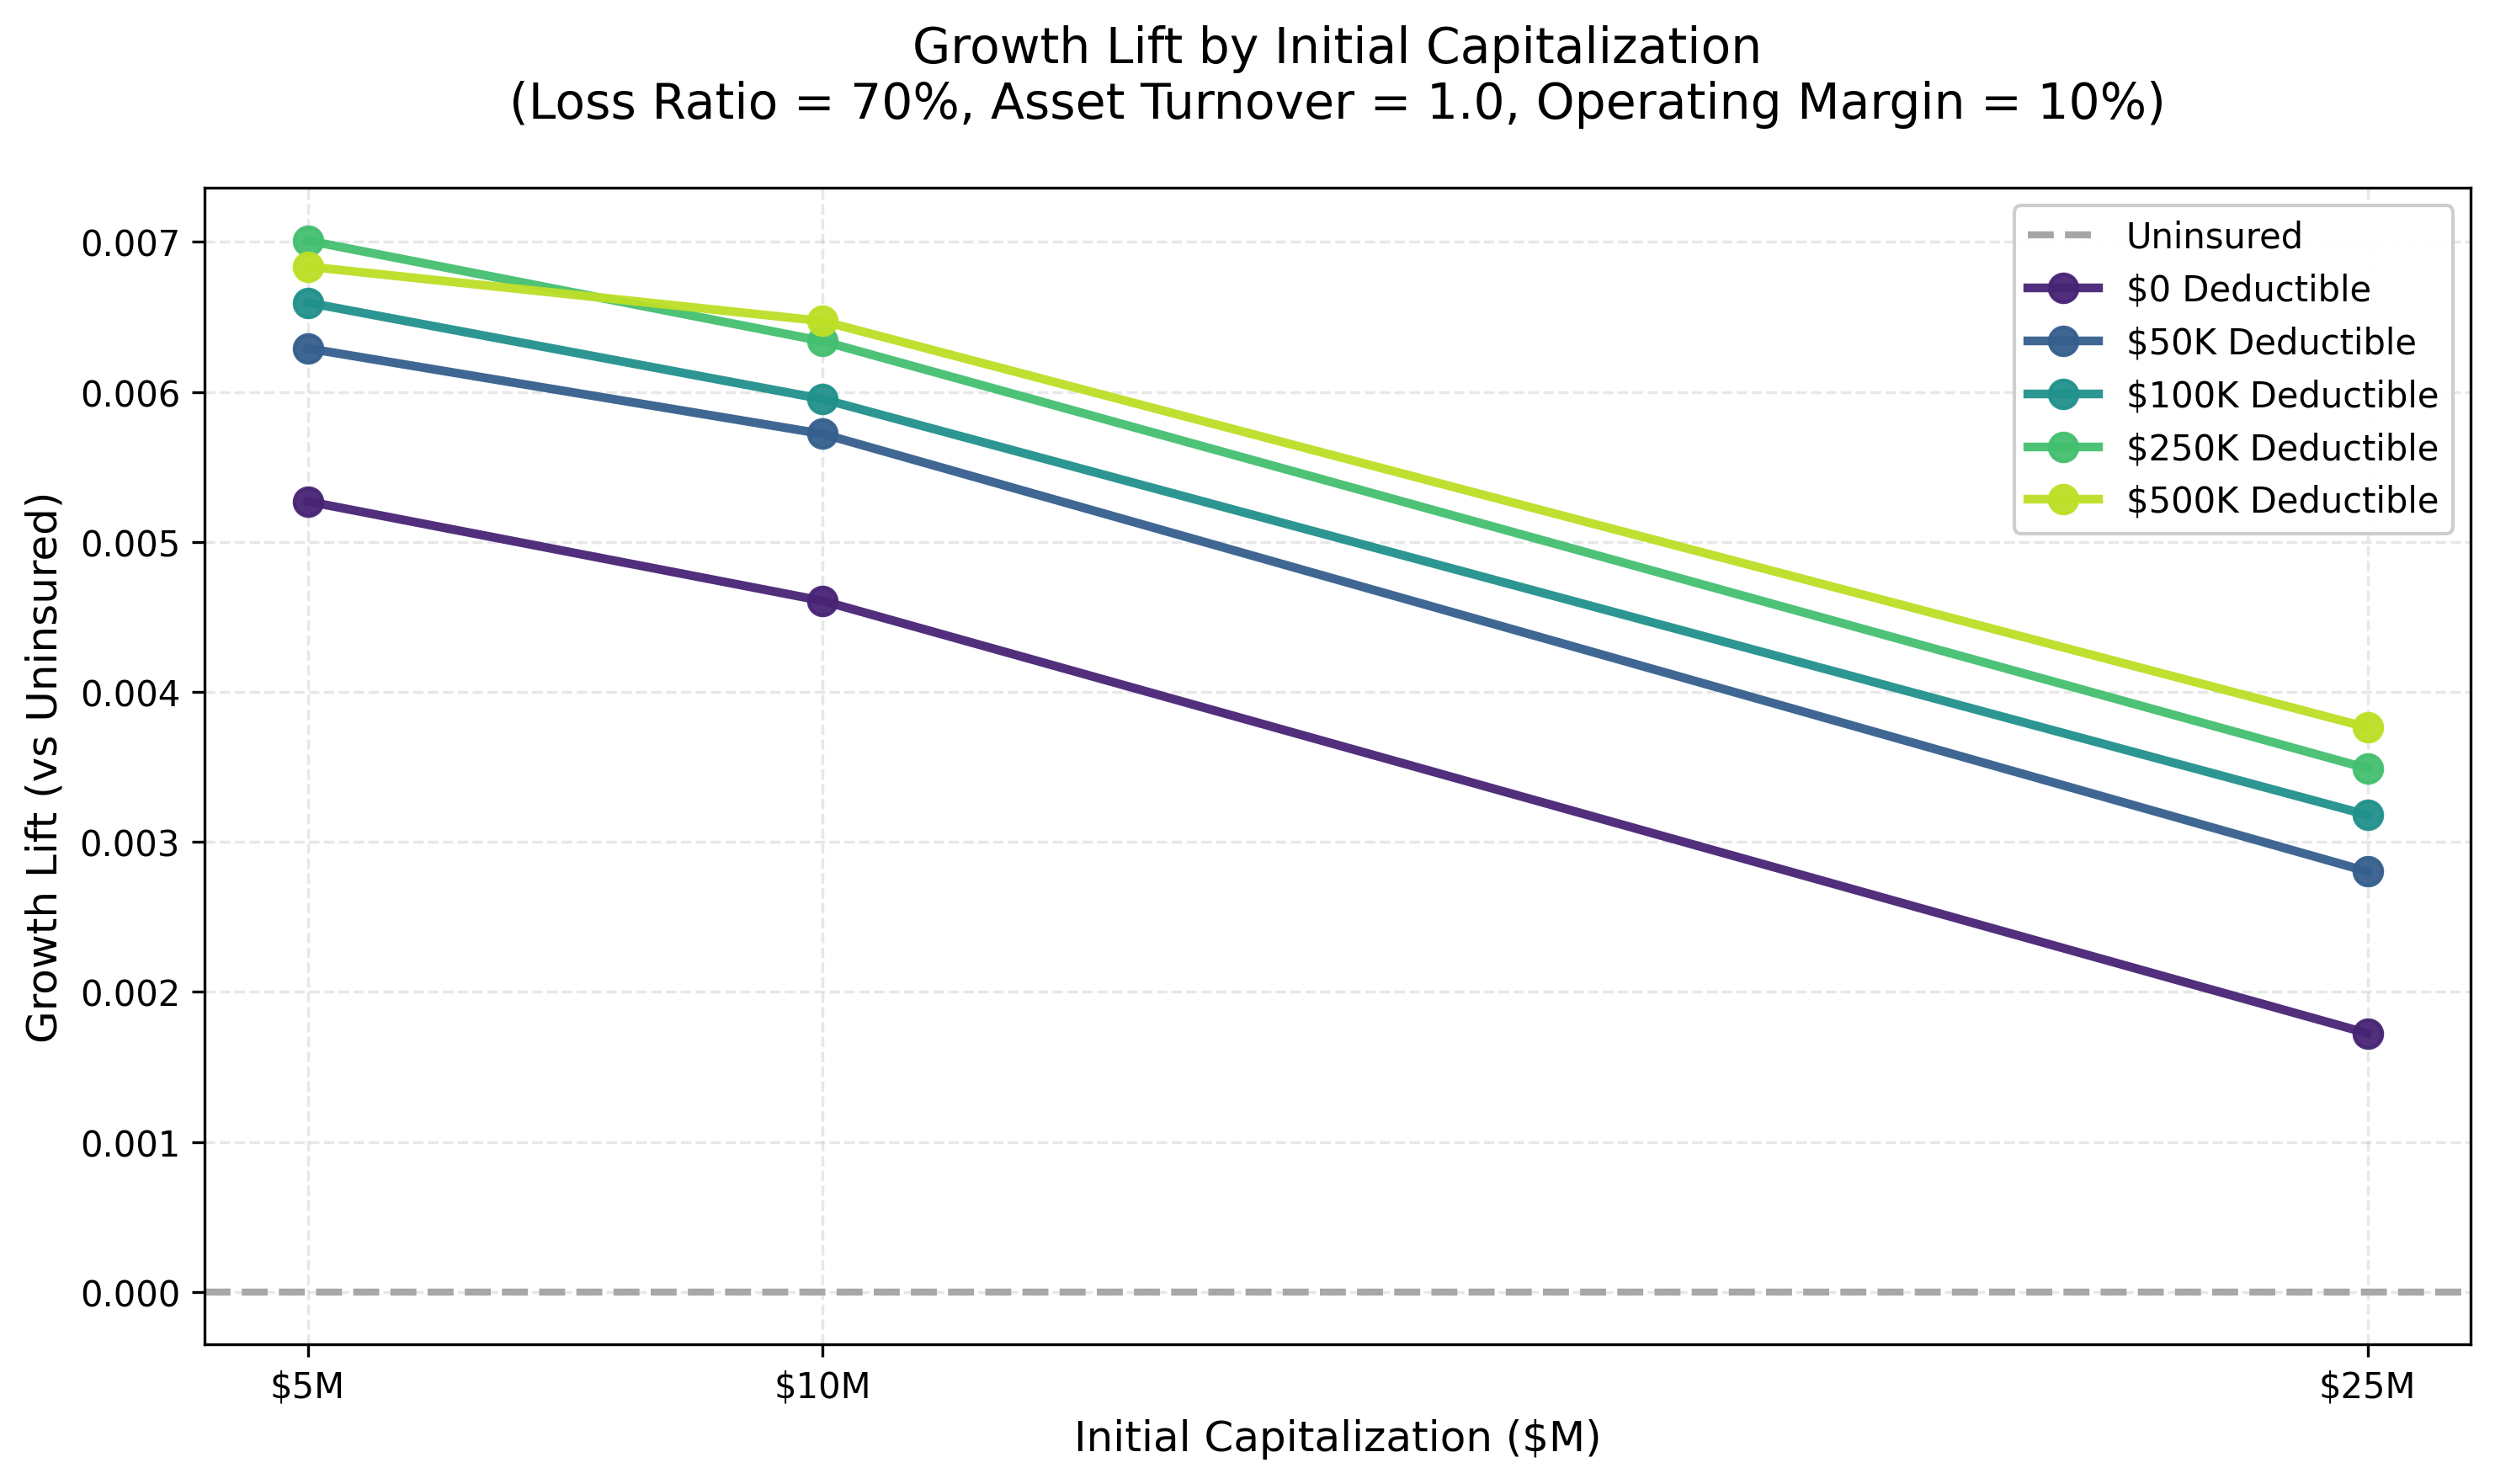
\includegraphics[width=1.0\textwidth]{images/growth_lift_by_capitalization.png}
    \caption{Impact of initial capitalization on time-average growth rate. Growth lift measures the improvement in time-average growth rate relative to self-insurance, quantifying the ergodic benefit of insurance.}
    \label{fig:growth_lift_by_cap}
\end{figure}

\textbf{Key Observations from Figure~\ref{fig:growth_lift_by_cap}:}

\textbf{Declining Insurance Value with Size:} Growth lift decreases systematically as capitalization increases. At \$5M capitalization, even a \$500K deductible provides approximately 0.70\% annual growth lift, while at \$25M, the same deductible yields only 0.38\% lift. This \emph{scale effect} reflects the diminishing proportional impact of fixed-severity losses as the capital base expands. A \$5M catastrophic loss represents 100\% of equity for the smallest company but only 20\% for the largest, fundamentally altering the multiplicative growth dynamics.

\vspace{\baselineskip}

\textbf{Optimal Deductible Migration:} The optimal deductible (highest growth lift) shifts from \$100K-\$250K at \$5M capitalization to \$500K at \$10M-\$25M capitalization under baseline parameters. This progression aligns with the theoretical framework (Section~2.3): as capital grows relative to expected loss severity, companies can profitably retain more risk, trading premium savings against manageable volatility increases.

\vspace{\baselineskip}

\textbf{The Guaranteed Cost Penalty:} Critically, the \$0 deductible (guaranteed cost) strategy consistently delivers the \emph{lowest} growth lift across all capitalization levels, despite eliminating retained loss volatility. This counterintuitive finding demonstrates that \emph{eliminating all retention is suboptimal}. The premium burden of full coverage destroys more growth through guaranteed costs than it preserves through variance reduction. For the \$25M company, guaranteed cost actually produces \emph{negative} growth lift relative to self-insurance in some parameter combinations (visible in later figures), meaning full insurance coverage destroys value compared to retaining all risk.

\vspace{\baselineskip}

\textbf{The Retention Sweet Spot:} All scenarios exhibit an interior optimum: some retention is superior to both guaranteed cost and self-insurance. This result emerges from balancing two opposing forces: (1) premium savings from higher deductibles, which compound favorably over time, and (2) protection from catastrophic losses that trigger the multiplicative decay described in Section~2.2. The simulation suggests that \emph{moderate retention strategies dominate the extremes} across a wide parameter space.

\vspace{\baselineskip}

\textbf{Self-Insurance Threshold:} While not shown in this figure, additional analysis reveals that at capitalizations exceeding \$50M with the modeled loss distributions, self-insurance begins to dominate all insured strategies. At such scale, the company effectively becomes its own insurer, with sufficient capital to absorb tail losses without material growth impairment. This threshold will vary significantly with loss distribution parameters and operating characteristics, reinforcing the need for company-specific simulation analysis.

\vspace{\baselineskip}

\textbf{Practical Implications:} For corporate decision-makers, these patterns suggest several considerations:
\begin{itemize}
    \item Small and mid-market companies (\$5M-\$25M capital) derive substantial value from insurance even at relatively high premium loadings
    \item Guaranteed cost programs should be questioned unless driven by non-economic factors (regulatory requirements, credit constraints, or other considerations not modeled here)
    \item The optimal retention level depends critically on company-specific capitalization relative to loss exposure, not industry benchmarks or broker conventions
    \item Companies approaching \$50M+ capitalization should rigorously evaluate whether traditional insurance programs remain economically justified
\end{itemize}

\subsection{The Asset Turnover Effect: Exposure Scaling and Insurance Value}

Figures~\ref{fig:multiples_ebit_0.100}, \ref{fig:multiples_ebit_0.125}, and~\ref{fig:multiples_ebit_0.150} display growth lift across asset turnover ratios (0.8 to 1.2) in a 3×3 grid format, with rows representing target loss ratios (60\%, 70\%, 80\%) and columns representing capitalization levels (\$5M, \$10M, \$25M). Each panel shows how growth lift varies with asset turnover for different deductible strategies.

\vspace{\baselineskip}

\textbf{Increasing Growth Lift with Turnover:} Within each panel, growth lift generally increases as asset turnover rises (moving right along the x-axis). This pattern is most pronounced at lower capitalizations and becomes muted or even reverses at \$25M. The mechanism driving this effect operates through the \emph{exposure scaling} built into the simulation framework: higher asset turnover generates proportionally more revenue, which increases loss frequency via the revenue-based exposure multiplier (Section~3.2, loss generation parameters).

When a company with 1.2 asset turnover generates 50\% more revenue than an otherwise-identical company with 0.8 turnover, it faces approximately 50\% more loss events annually. This increased loss frequency amplifies the \emph{frequency of multiplicative shocks} to the capital base, intensifying the non-ergodic dynamics that insurance mitigates. Consequently, insurance provides greater growth value to high-turnover operations because they experience more frequent opportunities for catastrophic losses to compound negatively over time.

\vspace{\baselineskip}

\textbf{Interaction with Capitalization:} The asset turnover effect weakens dramatically at higher capitalizations. For \$25M companies (rightmost column in each figure), growth lift often \emph{decreases} with turnover, and in some cases high deductibles and self-insurance converge or cross. This reversal occurs because larger capital bases can absorb the increased loss frequency without triggering the multiplicative decay that dominates smaller companies. Once capital substantially exceeds typical loss severity, additional exposure increases revenues (and thus potential growth) faster than it introduces material risk, reducing the relative value of insurance protection.

\vspace{\baselineskip}

\textbf{Practical Implications:} Efficient capital users generating substantial revenues relative to their balance sheet (i.e., companies with high asset turnover ratios) should recognize that they face disproportionately greater insurance value than low-turnover peers with similar capitalization. This suggests that focus should shift from absolute exposure size towards \emph{turnover-adjusted exposure intensity} that drives time-average growth dynamics.

\subsection{Operating Margin Interactions: The Profitability Buffer}

Comparing growth lift patterns across the three margin levels (Figures~\ref{fig:multiples_ebit_0.100}, \ref{fig:multiples_ebit_0.125}, and~\ref{fig:multiples_ebit_0.150}) reveals that higher operating margins systematically \emph{flatten} the response curves, reducing sensitivity to both asset turnover and insurance pricing variations.

\vspace{\baselineskip}

\textbf{The Margin Effect Mechanism:} Operating margins create a profitability buffer that dampens the impact of both insurance premiums and retained losses on growth rates. A company with 15\% operating margin can absorb a \$100K loss from a larger earnings base than an otherwise-identical company with 10\% margin, reducing the proportional impact on retained earnings and equity accumulation. Similarly, insurance premiums represent a smaller fraction of operating income for high-margin businesses, reducing the growth drag from premium costs.

Both asset turnover and operating margin contribute to earnings growth, but through different mechanisms: turnover by scaling revenue generation, and margin by improving profitability per dollar of revenue. When margins are high, the \emph{variance in outcomes across different insurance strategies diminishes} because the strong underlying profitability swamps the differential premium costs and retained loss distributions. Conversely, low-margin operations exhibit greater sensitivity to insurance choices because premiums and retained losses represent a larger fraction of net income, materially affecting growth trajectories.

\vspace{\baselineskip}

\textbf{Practical Implications:} Low-margin businesses (10\% or below before losses in this simulation, translating to about 5\% ensemble-average after losses) should pay particularly close attention to insurance optimization, as suboptimal strategies impose larger relative growth penalties. High-margin enterprises enjoy greater strategic flexibility: while optimal deductibles still exist, the growth differential between good and poor insurance decisions is smaller, potentially justifying simpler risk management approaches or greater emphasis on non-financial considerations (administrative burden, credit concerns, etc.).

\subsection{Sensitivity to Insurance Pricing: Loss Ratio Effects}

The row structure in Figures~\ref{fig:multiples_ebit_0.100}, \ref{fig:multiples_ebit_0.125}, and~\ref{fig:multiples_ebit_0.150} isolates the impact of target loss ratios (60\%, 70\%, 80\%), representing the insurer's pricing efficiency. Lower loss ratios indicate higher expense loadings and profit margins, making insurance more expensive for the buyer.

\vspace{\baselineskip}

\textbf{Pricing Impact on Growth Lift:} As expected, cheaper insurance (higher loss ratios, lower rows in each figure) produces substantially greater growth lift. At 80\% loss ratio (bottom row), even guaranteed cost (\$0 deductible) frequently exceeds the growth rate of self-insurance for \$5M and \$10M capitalizations, while at 60\% loss ratio (top row), only moderate-to-high deductibles remain attractive. This pattern confirms the theoretical prediction that insurance creates value through variance reduction, but excessive premium costs can overwhelm this benefit.

\vspace{\baselineskip}

\textbf{Robustness at Lower Capitalizations:} Critically, even at the \emph{expensive} 60\% loss ratio, insurance still delivers substantial growth lift for \$5M capitalization across nearly all deductible levels and turnover ratios. This robustness demonstrates that the ergodic benefit of reducing multiplicative volatility can justify significant premium loadings when capital is scarce relative to potential losses. For small companies, insurance remains economically rational even when premiums substantially exceed actuarially fair rates (a finding invisible to traditional expected value analysis).

\vspace{\baselineskip}

\textbf{Optimal Deductible Sensitivity:} Cheaper insurance (higher loss ratios) shifts optimal deductibles lower. At 80\% loss ratio, \$50K-\$100K deductibles often maximize growth lift even for \$10M companies, while at 60\% loss ratio, \$250K-\$500K deductibles dominate. This migration reflects the changing trade-off between premium savings and volatility protection: when insurance is expensive, companies must retain more risk to avoid excessive premium burden; when insurance is cheap, lower deductibles become attractive because the marginal premium cost of additional coverage is modest.

\vspace{\baselineskip}

\textbf{Practical Implications:} Corporate buyers should actively estimate loss costs and negotiate loss ratios, as pricing efficiency directly determines optimal retention strategies and realized growth lift. The substantial variation in growth outcomes across loss ratio scenarios suggests that \emph{insurance market cycles} (not modeled here) may create significant timing opportunities: companies purchasing programs during soft markets (high loss ratios) can justify lower deductibles, while hard markets (low loss ratios) favor higher retentions.

\subsection{Limitations and Boundary Conditions}

While the simulation results provide valuable directional insights, several important limitations constrain their generalizability. Corporate decision-makers should carefully consider whether their specific circumstances violate key modeling assumptions:

\vspace{\baselineskip}

\textbf{Frequency Tail Correlations:} The Poisson loss frequency assumption implies that high volumes of attritional losses below the deductible are extremely rare and statistically independent. In reality, many operational risks exhibit clustering, as adverse years produce multiple related losses (e.g., supply chain disruptions, product liability waves, regulatory actions). Such correlation would increase the volatility of retained losses, potentially shifting optimal deductibles lower than the simulation suggests and making guaranteed cost strategies more attractive. Companies with known loss correlation patterns should adjust their expectations accordingly.

\vspace{\baselineskip}

\textbf{Regulatory Capital Requirements:} The model does not incorporate regulatory capital requirements, rating agency capital adequacy standards, or debt covenant restrictions that may impose binding constraints on retention decisions. For publicly traded companies, regulated entities, or leveraged businesses, these external constraints may override growth optimization considerations, forcing lower retentions than the ergodic analysis would recommend. The \emph{shadow price} of regulatory capital can be substantial, potentially reversing the guaranteed cost penalty observed here.

\vspace{\baselineskip}

\textbf{Credit and Liquidity Constraints:} The Letter of Credit mechanism assumes companies can costlessly post collateral at 1.5\% annually and face no liquidity constraints. Real companies face:
\begin{itemize}
    \item Higher collateral costs or limited credit facility capacity, increasing the effective retention cost
    \item Cash flow constraints that make large retained losses operationally disruptive, even if balance sheet equity remains positive
    \item Credit rating impacts from reserve increases, raising borrowing costs and limiting growth opportunities
\end{itemize}

These frictions would increase the value of insurance beyond the modeled growth lift, particularly for companies with tight credit conditions or those relying on external financing for growth.

\vspace{\baselineskip}

\textbf{Other Unmodeled Factors:} Additional considerations that may affect real-world insurance decisions include:
\begin{itemize}
    \item \textbf{Loss control and risk engineering services} provided by insurers, which may reduce expected losses beyond the pure financial transfer
    \item \textbf{Claims handling expertise} that insurers provide, particularly for complex liability or litigation-intensive exposures
    \item \textbf{Tax asymmetries} beyond the basic corporate rate modeled (e.g., loss carryforward limitations, alternative minimum tax)
    \item \textbf{Stakeholder preferences} from boards, shareholders, or management with non-growth objectives (e.g., earnings stability, dividend consistency)
    \item \textbf{Competitive and strategic considerations} where financial distress creates market share losses or acquisition vulnerability
\end{itemize}

\vspace{\baselineskip}

\textbf{Recommendations for Application:} Given these limitations, practitioners should view the simulation results as \emph{directional guidance} rather than prescriptive recommendations. The optimal strategy for any specific company requires:
\begin{enumerate}
    \item \textbf{Custom loss distribution calibration} using company-specific historical data, industry benchmarks, and exposure analysis
    \item \textbf{Incorporation of company-specific constraints} including regulatory capital, credit facilities, and stakeholder requirements
    \item \textbf{Sensitivity analysis} across parameter uncertainty ranges, particularly for catastrophic loss tail parameters
    \item \textbf{Scenario testing} for correlated loss events, market cycle dynamics, and business strategy changes
\end{enumerate}

The simulation framework provides the analytical foundation for such company-specific analyses. CFOs, risk managers, and actuaries are encouraged to adapt the methodology to their particular circumstances rather than applying the illustrated results directly.

\begin{figure}[htbp]
    \centering
    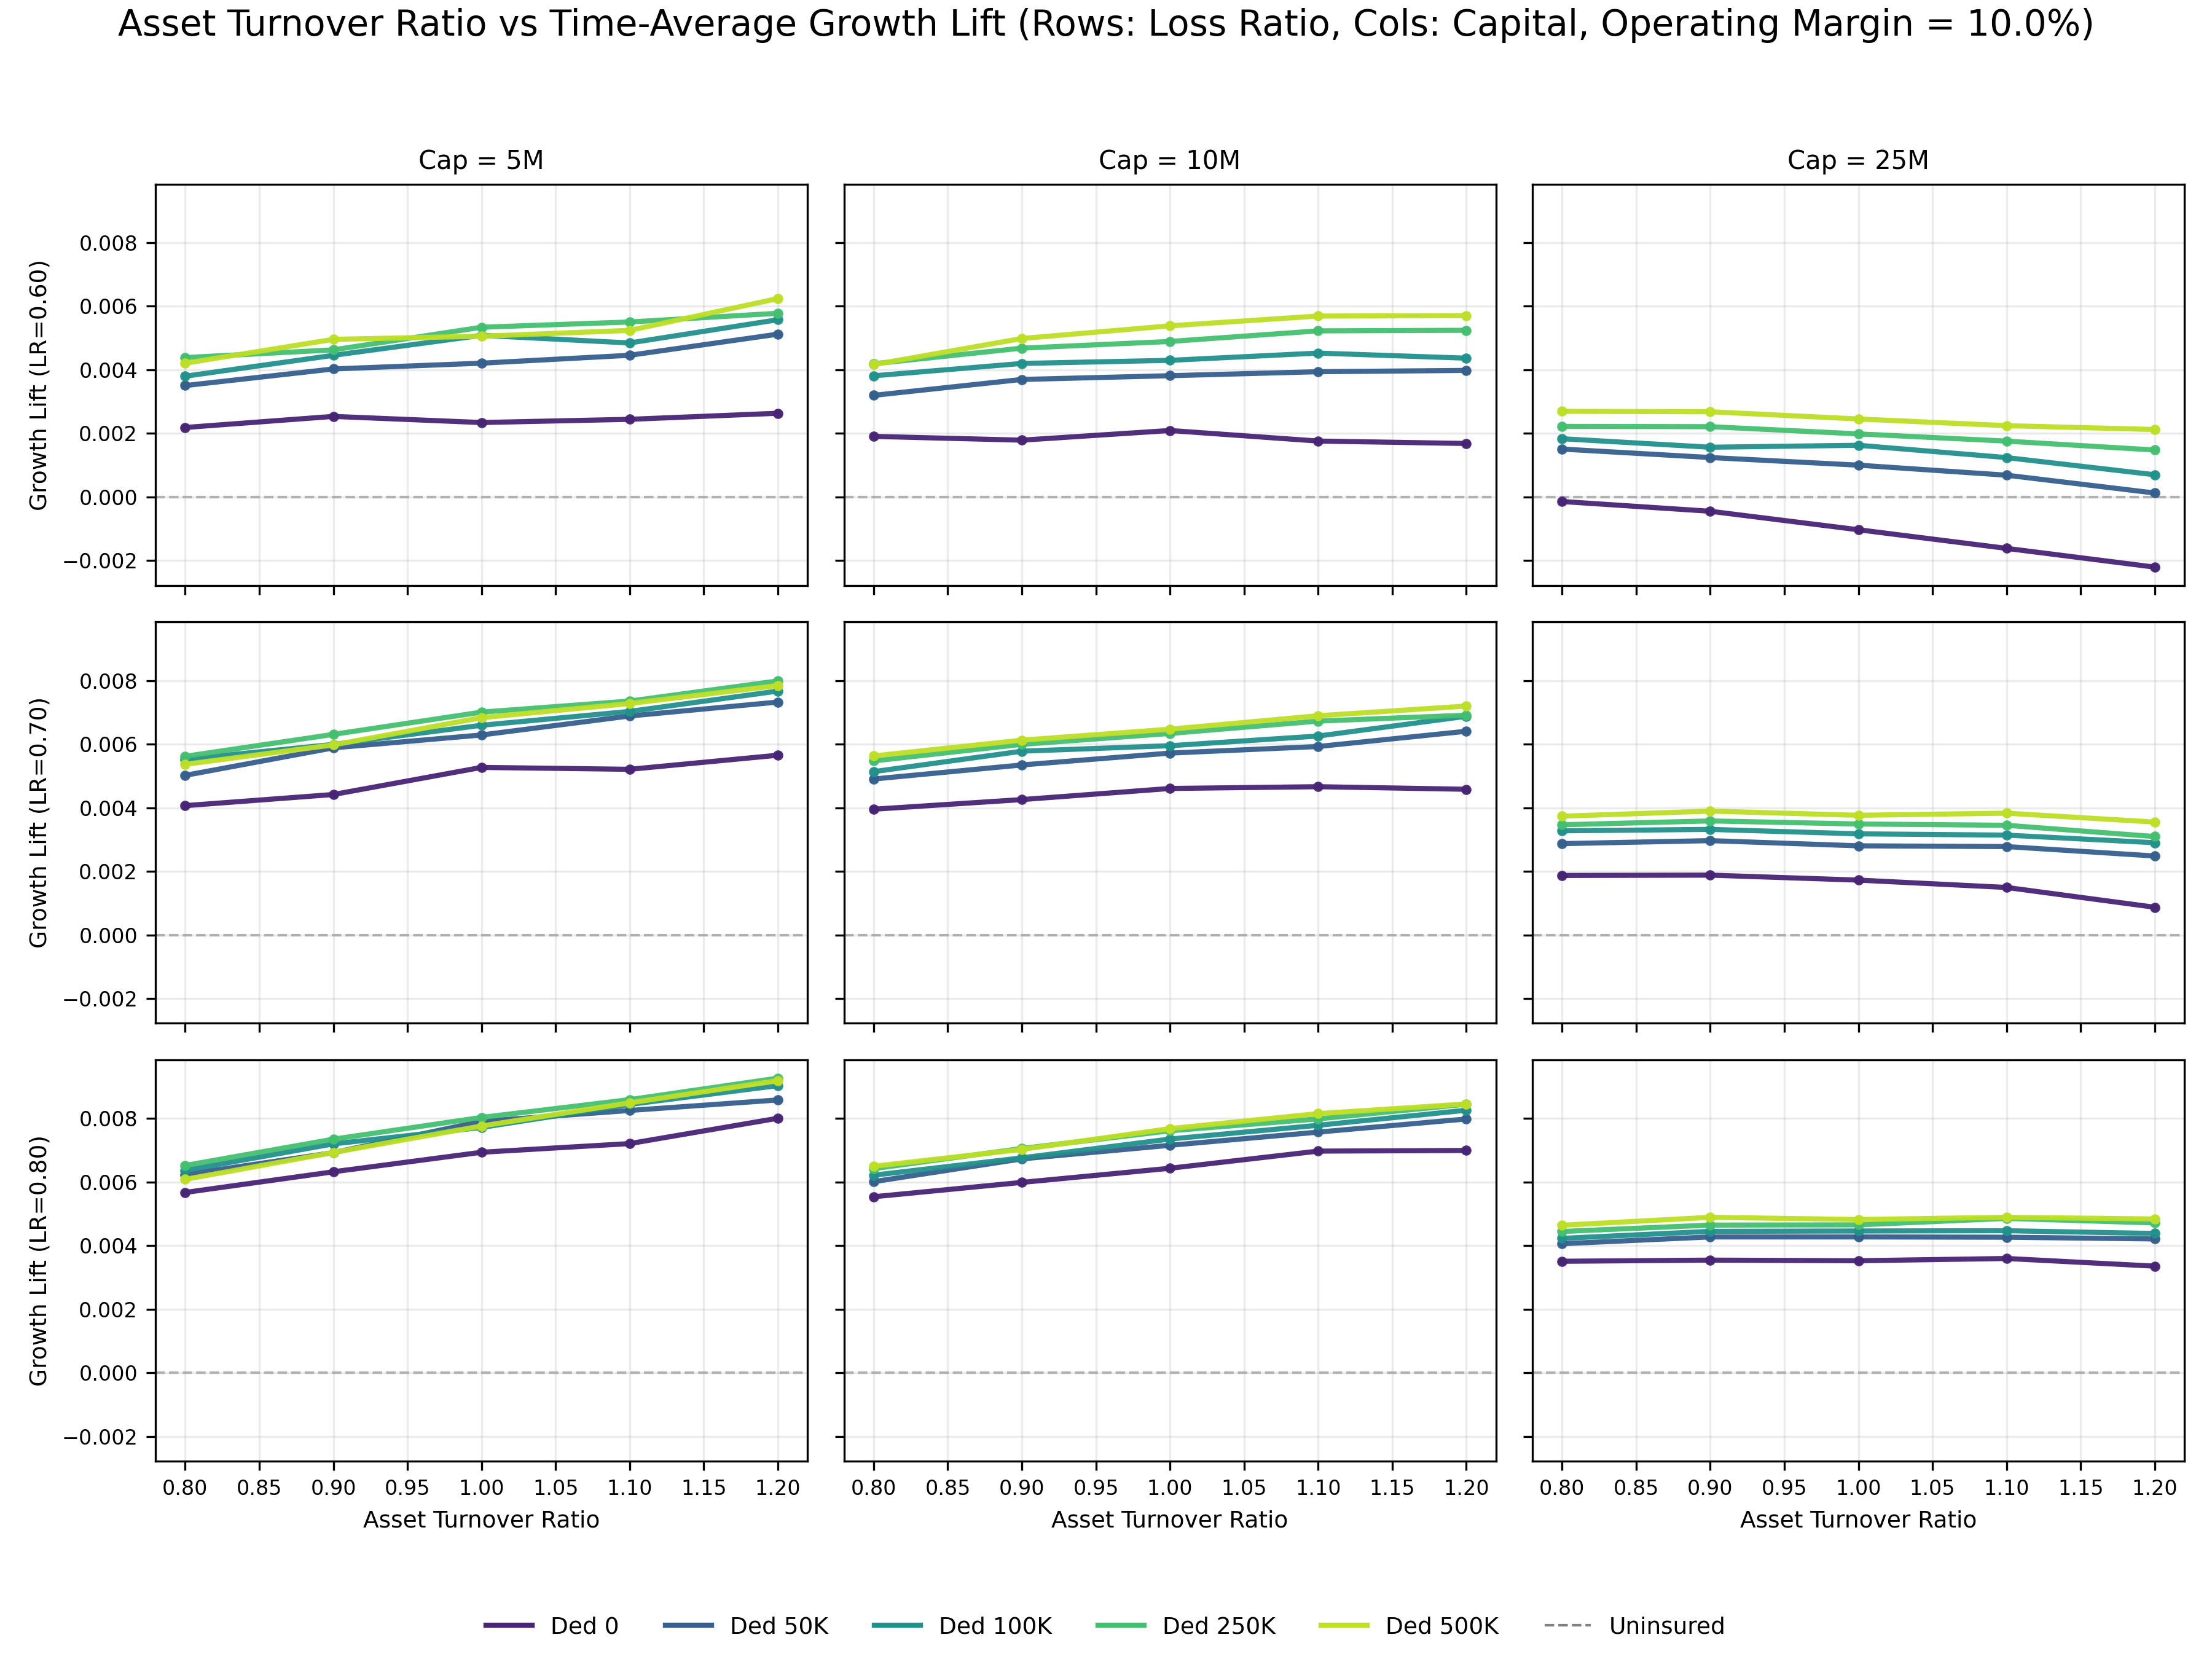
\includegraphics[width=1.0\textwidth]{images/option3_multiples_ebit_0.100.png}
    \caption{Impact of asset turnover ratio on time-average growth rate at operating margin of 10\%.}
    \label{fig:multiples_ebit_0.100}
\end{figure}

\begin{figure}[htbp]
    \centering
    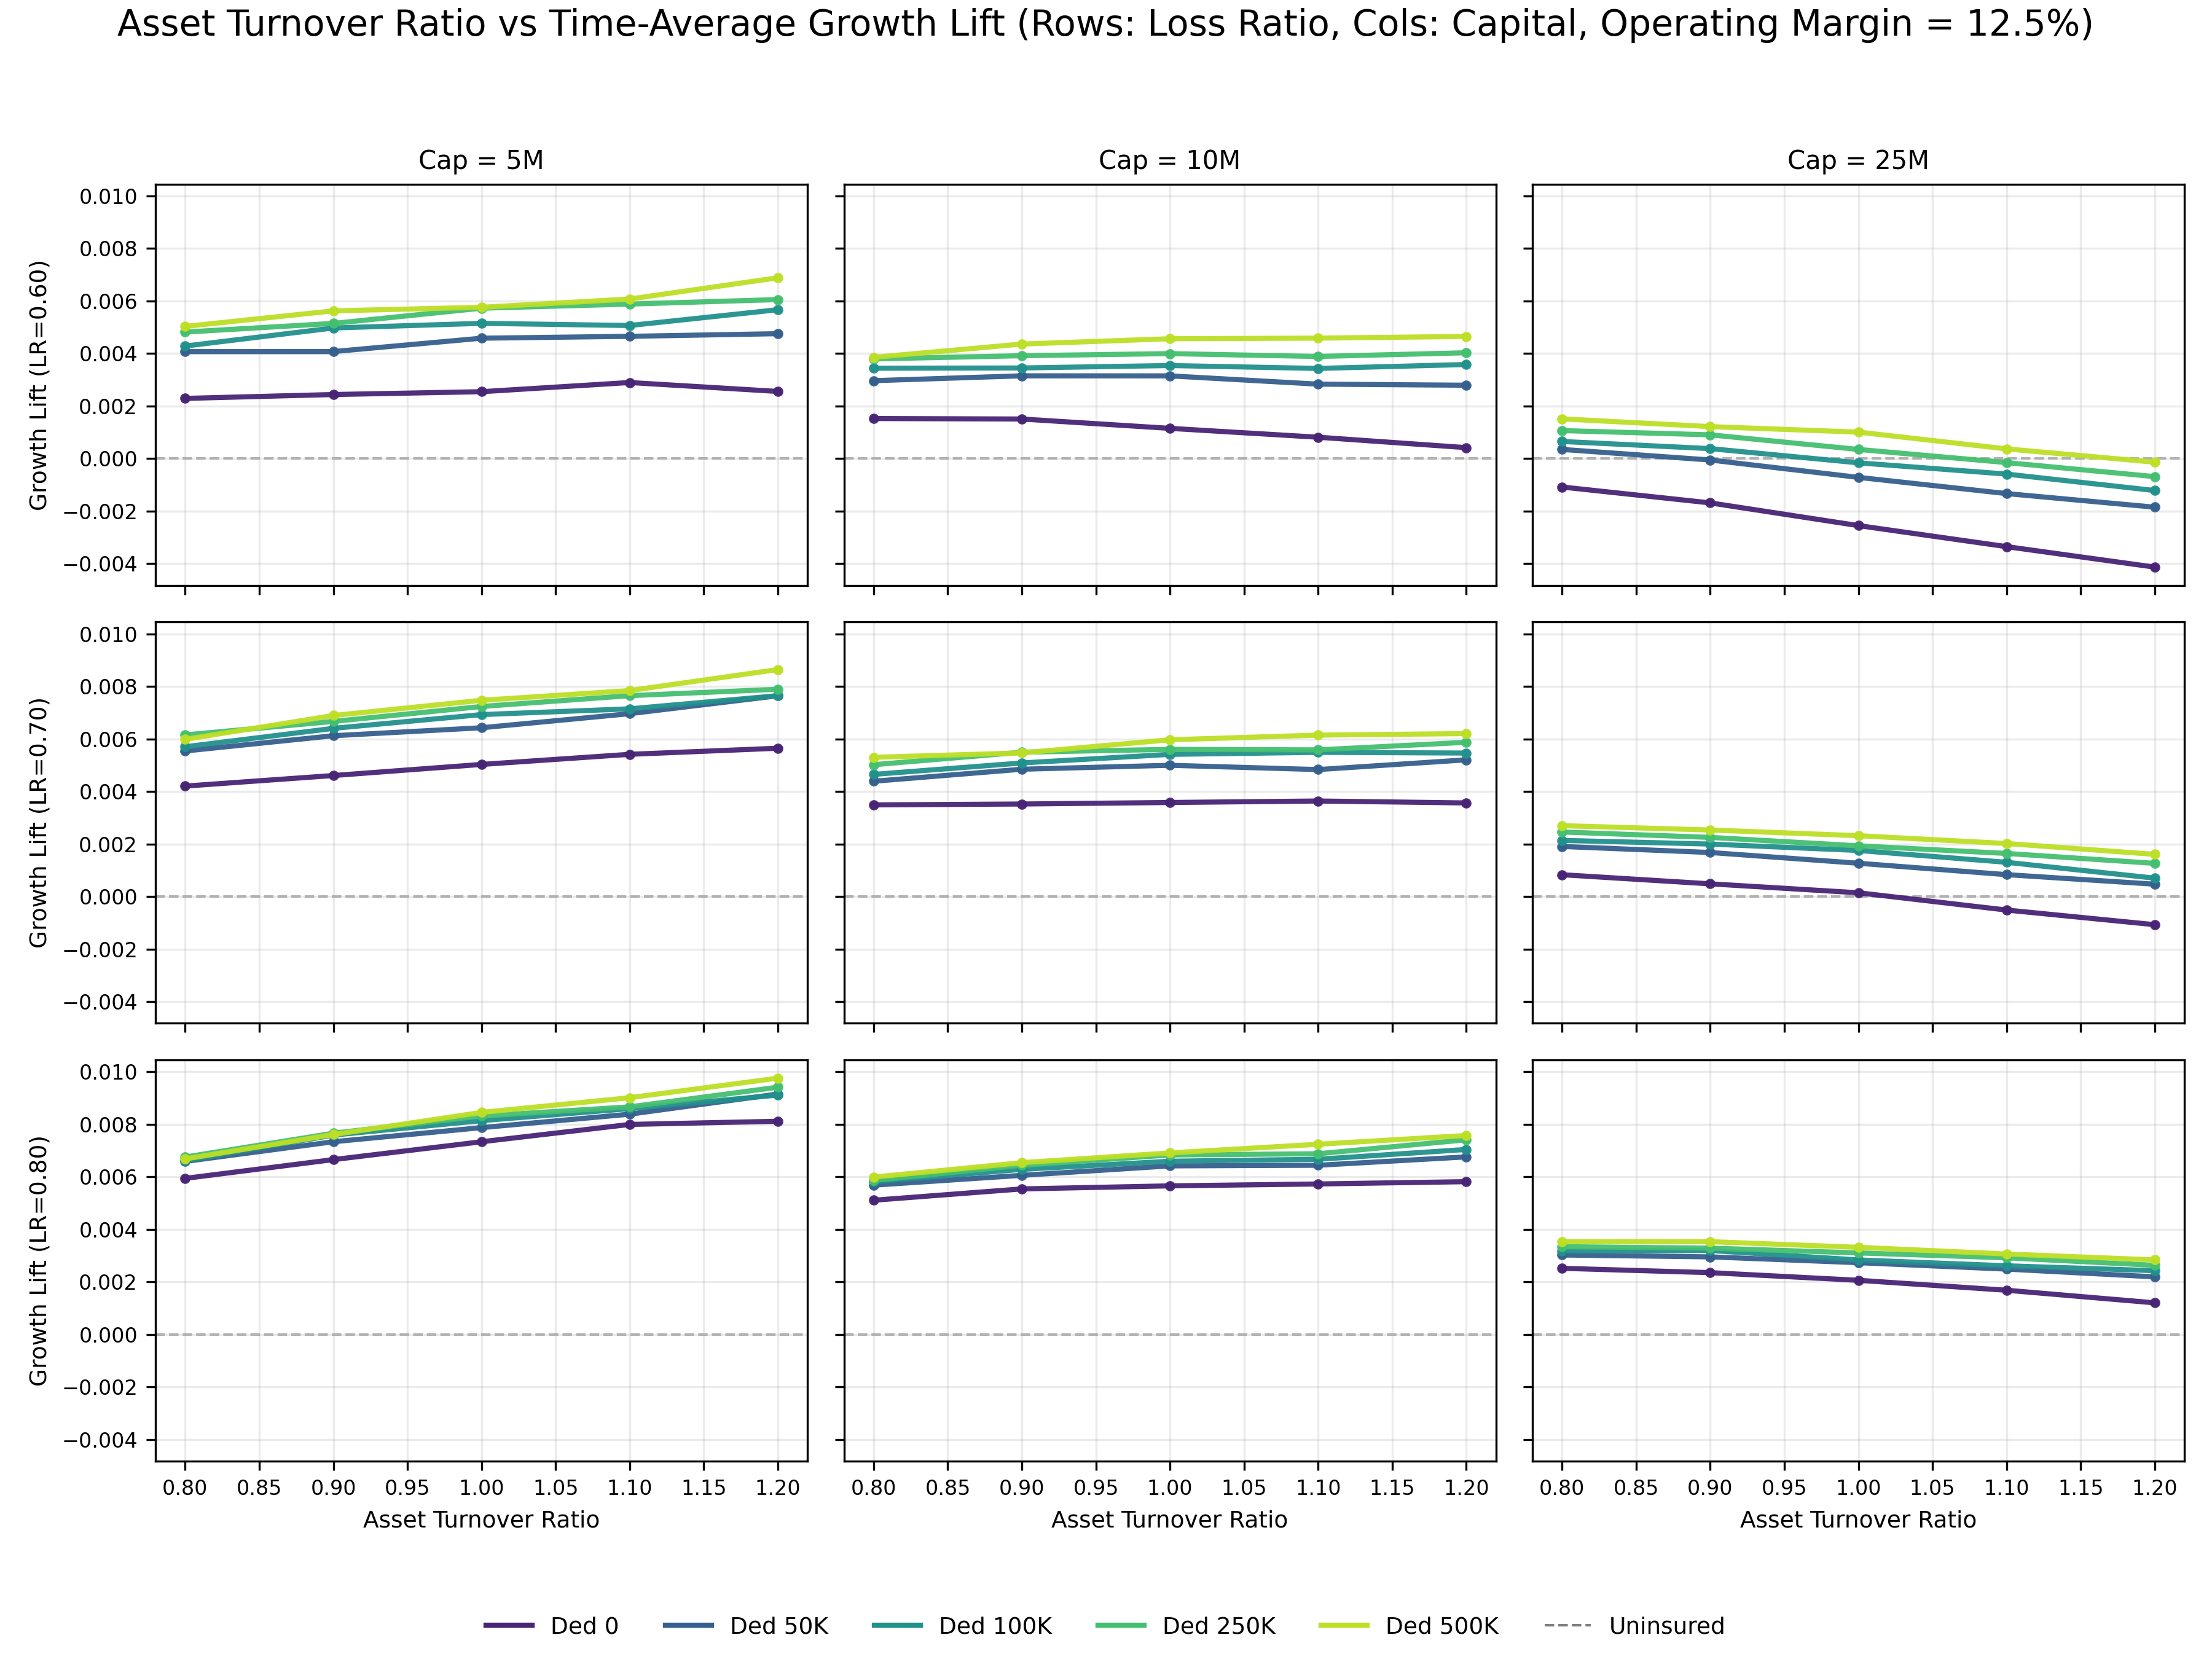
\includegraphics[width=1.0\textwidth]{images/option3_multiples_ebit_0.125.png}
    \caption{Impact of asset turnover ratio on time-average growth rate at operating margin of 12.5\%.}
    \label{fig:multiples_ebit_0.125}
\end{figure}

\begin{figure}[htbp]
    \centering
    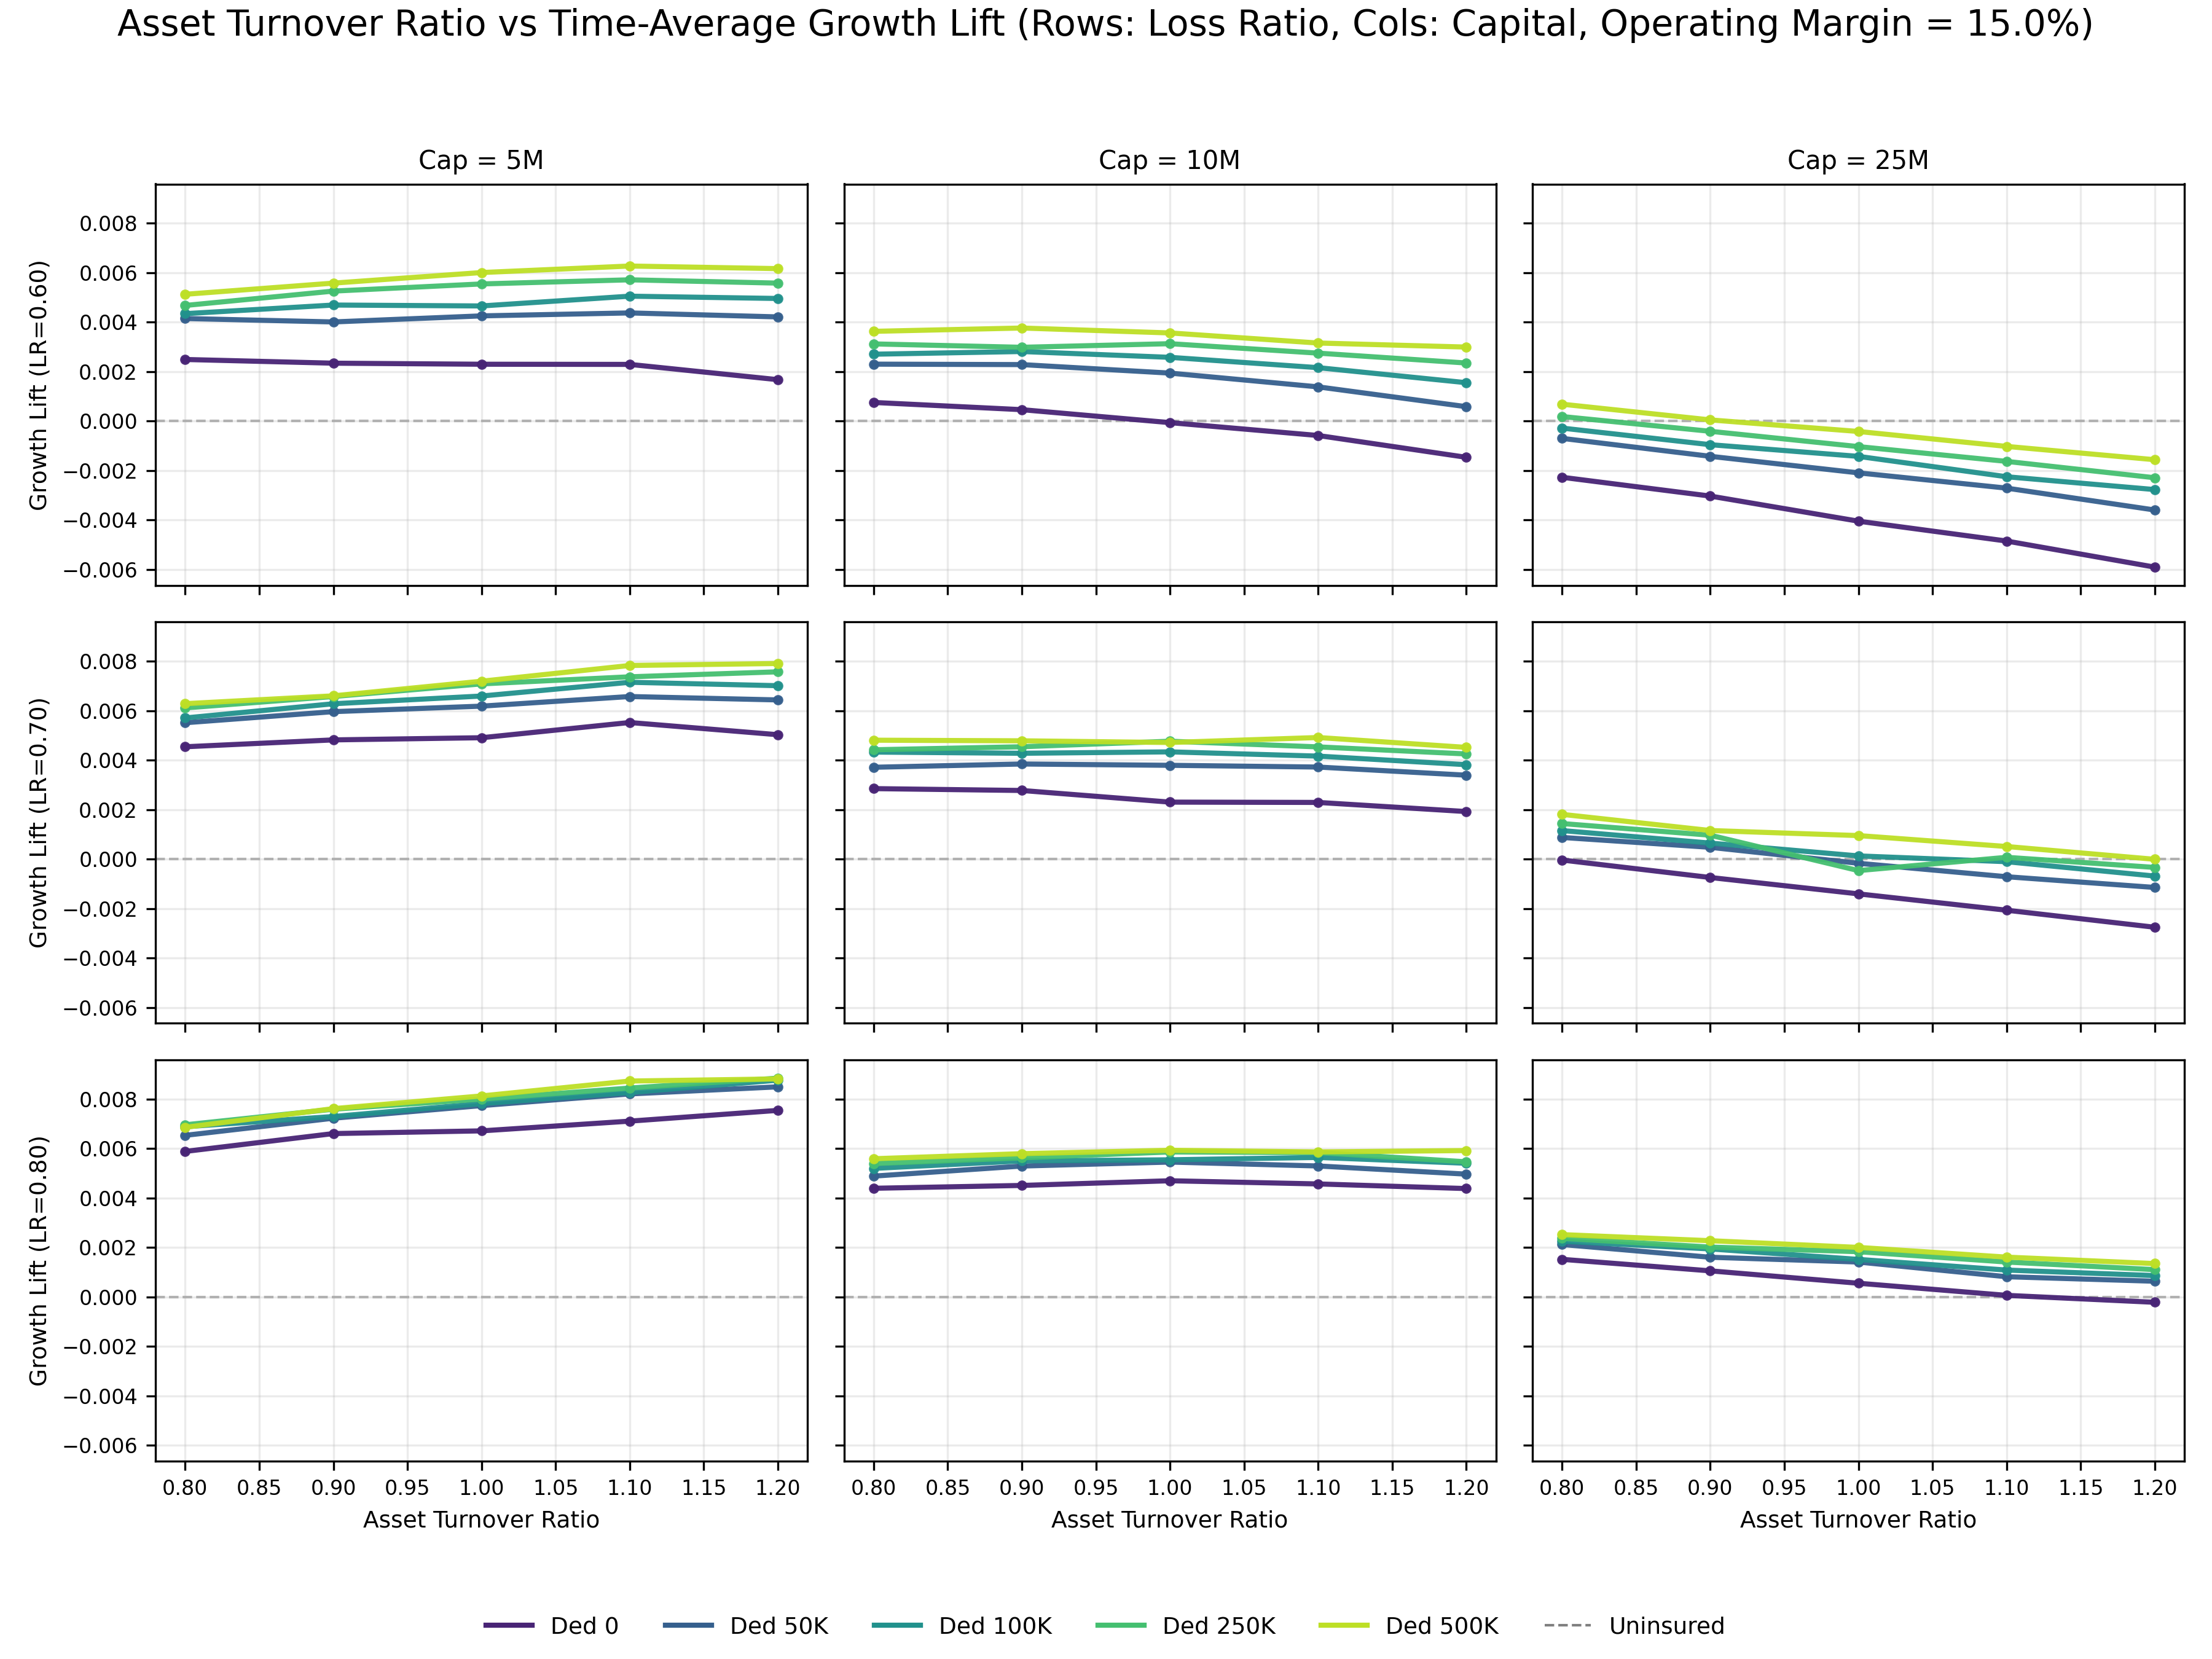
\includegraphics[width=1.0\textwidth]{images/option3_multiples_ebit_0.150.png}
    \caption{Impact of asset turnover ratio on time-average growth rate at operating margin of 15\%.}
    \label{fig:multiples_ebit_0.150}
\end{figure}

\section{Implications for Insurance Decision-Making}

\subsection{Reframing Insurance Value Through Time Averages}

The ergodic perspective fundamentally changes how corporate decision-makers should evaluate insurance. Rather than focusing on expected values and traditional cost-benefit analyses, risk managers must consider the time-average growth rate experienced by their specific company over its operational horizon. This shift reveals that insurance premiums substantially exceeding expected losses can still enhance long-term value creation by reducing the multiplicative impact of catastrophic events.

\subsection{The Ergodic Perspective on Risk Retention}

The simulation demonstrates that some level of risk retention is consistently optimal, challenging both full insurance and complete self-insurance strategies. This finding emerges from the ergodic framework's recognition that predictable attritional losses should be retained while catastrophic tail risks require transfer. The optimal retention level balances premium savings against the growth-destroying potential of large losses.

\subsection{Company Profile Considerations}

\textbf{Important Note:} The specific results presented in this paper are illustrative and depend heavily on the modeled loss distributions, business parameters, and simplifying assumptions. Corporate decision-makers should not apply these findings directly but rather use them as motivation to conduct company-specific ergodic analysis.

Key considerations emerging from the simulation include the critical role of capitalization levels, operating margin buffers, and loss severity distributions in determining optimal insurance strategies. Companies with lower capitalizations relative to potential losses derive substantially more value from insurance, even at higher premium rates.

\subsection{Engaging Actuarial Expertise for Ergodic Analysis}

CFOs and risk managers should engage experienced actuaries to model time-dependent paths specific to their industry and company characteristics. Traditional actuarial analysis focusing on expected values and ensemble statistics may systematically undervalue insurance for growth-focused companies. The actuarial profession must evolve to incorporate ergodic considerations into standard practice, developing new tools and methodologies for time-average optimization.

\subsection{Challenging Traditional Risk Management Metrics}

Standard risk metrics such as Value at Risk (VaR) and Expected Shortfall fail to capture the multiplicative nature of wealth dynamics and the critical distinction between time and ensemble averages. Risk management frameworks must evolve to incorporate ergodic considerations, particularly for long-term strategic decisions where path dependence and growth optimization matter more than short-term volatility measures.

\section{Future Research Directions}

This initial exploration of ergodic insurance optimization reveals numerous opportunities for extending the framework to address current model limitations and enhance practical applicability.

\subsection{Optimizing Complex Insurance Structures}

The current model's simplification to deductible-only structures masks important optimization opportunities in real-world insurance programs. Future research should incorporate:
\begin{itemize}
    \item Multi-layer tower structures with different attachment points and limits
    \item Aggregate deductibles and limits that recognize claim correlation
    \item Reinstatement provisions and their impact on tail risk protection
    \item Coverage sub-limits by peril or location
\end{itemize}

These extensions would enable practitioners to optimize complete insurance programs rather than single-parameter deductibles.

\subsection{Dynamic and Adaptive Insurance Strategies}

Static insurance decisions fail to capture the dynamic nature of business growth and market evolution. Future work should develop:
\begin{itemize}
    \item Adaptive strategies that adjust coverage as companies grow
    \item Market-responsive approaches that capitalize on insurance pricing cycles
    \item Path-dependent optimization recognizing that insurance decisions affect future growth trajectories
    \item Switching costs and multi-year contract considerations
\end{itemize}

\subsection{Incorporating Loss Correlations and Portfolio Effects}

The independence assumption for losses oversimplifies real risk landscapes. Extensions should model:
\begin{itemize}
    \item Correlation between different loss types and business lines
    \item Diversification benefits in multi-line enterprises
    \item Systemic risks and contagion effects
    \item Natural hedging opportunities within business portfolios
\end{itemize}

\subsection{Stochastic Business and Market Dynamics}

The deterministic revenue and margin assumptions limit the model's realism. Future research should incorporate:
\begin{itemize}
    \item Inflation, discounting, and time value of money
    \item Revenue volatility and its interaction with insurance value
    \item Economic cycles affecting both business performance and loss frequencies
    \item Insurance market cycles and their impact on optimal retention
    \item Competitive dynamics and market share considerations
\end{itemize}

\subsection{Industry-Specific Applications and Regulatory Considerations}

The generic manufacturing model requires specialization for practical implementation:
\begin{itemize}
    \item Industry-specific loss distributions and exposure bases
    \item Regulatory capital requirements and their optimization
    \item Rating agency considerations and cost of capital impacts
    \item Sector-specific risk factors (e.g., cyber for technology, liability for healthcare)
\end{itemize}

These extensions would transform the framework from an illustrative model to a practical decision support tool for corporate risk management.

\section{Conclusion}

This white paper has introduced a novel simulation framework based on ergodicity economics principles for analyzing insurance risk appetite. Our key findings demonstrate that company size significantly influences risk appetite, with larger insurers exhibiting greater willingness to underwrite risk. This finding has important implications for competitive dynamics and market structure in P\&C insurance.

The simulation framework provides a powerful tool for:
\begin{itemize}
    \item Understanding temporal risk dynamics
    \item Optimizing portfolio decisions
    \item Informing strategic planning
\end{itemize}

I encourage industry practitioners to explore these concepts further and welcome collaboration on extending this research.

The framework will provide new insights for companies making insurance decisions and is intended to answer questions such as "what is the ROI of our insurance program?", "how much insurance do we need?" and considerations of optimal insurance deductibles and limits.

% Bibliography
\bibliographystyle{apalike}
\bibliography{references}

\pagebreak

% Appendices
\appendix
\section{Technical Appendix}

\subsection{Simulation Algorithm Details}

This appendix provides algorithmic details for the core simulation engine, with emphasis on the timing of financial statement updates, insurance claim payments, and premium recognition. Readers interested in full implementation details should consult the GitHub repository referenced in Section~\ref{sec:code-repo}.

\subsubsection{Annual Simulation Loop}

The simulation executes a discrete-time loop over the specified horizon $T$ (50 years in this case), generating loss events and updating financial state at annual intervals. The high-level algorithm proceeds as follows:

\begin{algorithmic}[1]
\State \textbf{Initialize:} $t \gets 0$, Assets$_0 \gets$ initial capital, Equity$_0 \gets$ Assets$_0$
\State \textbf{Initialize:} Outstanding claims $\mathcal{C} \gets \emptyset$
\While{$t < T$ \textbf{and} Equity$_t > 0$}
    \State Generate loss events $L_t$ from three-tier loss distribution (see Section~\ref{sec:loss-gen})
    \For{each loss $\ell \in L_t$}
        \State Allocate $\ell$ between company retention and insurance recovery
        \State Create claim liability with 10-year payment schedule
        \State Post collateral for company portion: Collateral $\gets$ Collateral $+$ retention($\ell$)
    \EndFor
    \State Calculate revenue: $R_t \gets \text{Assets}_t \times \text{TurnoverRatio}$
    \State Calculate operating income: $\text{EBIT}_t \gets R_t \times \text{Margin} - \text{Premiums}_t - \text{Depreciation}_t \text{ (always 0)}$
    \State Process scheduled claim payments from $\mathcal{C}$ (Algorithm~\ref{alg:claim-payments})
    \State Calculate net income: $\text{NI}_t \gets (\text{EBIT}_t - \text{Losses}_t) \times (1 - \tau)$ \text{ (where } $\tau$ \text{ is the tax rate)}
    \State Update equity: Equity$_{t+1} \gets$ Equity$_t +$ NI$_t \times \rho$ (where $\rho$ is the retention ratio)
    \State Update assets: Assets$_{t+1} \gets$ Equity$_{t+1} +$ Liabilities$_{t+1}$
    \State $t \gets t + 1$
\EndWhile
\State \textbf{Return:} Time series $\{\text{Assets}_t, \text{Equity}_t, \text{Revenue}_t, \text{ROE}_t\}_{t=0}^{T}$
\end{algorithmic}

The simulation terminates upon insolvency (Equity$_t \leq 0$) or completion of the time horizon. The time-average growth rate for each trajectory is calculated as:
\begin{equation}
g_{\text{time}} = \frac{1}{T} \ln\left(\frac{\text{Equity}_T}{\text{Equity}_0}\right)
\end{equation}

This logarithmic formulation captures the multiplicative nature of wealth evolution and forms the basis for ergodic analysis across Monte Carlo scenarios.

\subsubsection{Balance Sheet Update Mechanism}

The annual \texttt{step()} method orchestrates financial statement updates with careful attention to the sequence of operations. The order is critical because each calculation affects subsequent balance sheet items. The method follows this sequence:

\begin{algorithmic}[1]
\State \textbf{Input:} Current balance sheet state, working capital percentage $w$, LoC rate $r_{\text{LoC}}$
\State \textbf{Step 1: Revenue Calculation}
\State Adjust for working capital: $A_{\text{eff}} \gets \frac{\text{Assets}}{1 + \text{Turnover} \times w}$ \text{ (}$w$ \text{is 0\% in this experiment)}
\State Calculate revenue: $R \gets A_{\text{eff}} \times \text{TurnoverRatio}$
\State \textbf{Step 2: Operating Income}
\State Calculate base operating income: $\text{EBIT}_{\text{base}} \gets R \times \text{OperatingMargin}$
\State Subtract insurance premiums: $\text{EBIT} \gets \text{EBIT}_{\text{base}} - \text{Premiums}$
\State Subtract depreciation: $\text{EBIT} \gets \text{EBIT} - \text{Depreciation (0 in this experiment)}$
\State \textbf{Step 3: Claim Payments and Collateral}
\State Process scheduled payments: \{payments, collateral released\} $\gets$ \texttt{pay\_claim\_liabilities()}
\State Accrue letter of credit charges: $\text{LoC\_cost} \gets \text{Collateral} \times r_{\text{LoC}}$
\State Record insurance losses for tax purposes: $\text{LossesPaid} \gets$ sum(payments)
\State \textbf{Step 4: Net Income}
\State Taxable income: $\text{TI} \gets \text{EBIT} - \text{LossesPaid} - \text{LoC\_cost}$
\State Net income: $\text{NI} \gets \text{TI} \times (1 - \tau)$
\State \textbf{Step 5: Balance Sheet Update}
\State Retained earnings: $\text{RE} \gets \text{NI} \times \rho$
\State Update equity: Equity$_{\text{new}} \gets$ Equity$_{\text{old}} + \text{RE}$
\State Update assets: Assets$_{\text{new}} \gets$ Equity$_{\text{new}} + $ Liabilities
\State \textbf{Return:} Metrics dictionary \{assets, equity, roe, revenue, net\_income, ...\}
\end{algorithmic}

\vspace{\baselineskip}

Key equations implemented in this sequence:

\vspace{\baselineskip}

\textbf{Operating Income:}
\begin{equation}
\text{EBIT} = R \times m - \text{Premiums} - \text{Depreciation}
\end{equation}
where $m$ is the base operating margin. Insurance premiums are treated as operating expenses, consistent with their role in the core business model.

\vspace{\baselineskip}

\textbf{Net Income and Equity Growth:}
\begin{equation}
\text{Equity}_{t+1} = \text{Equity}_t + (\text{EBIT}_t - \text{LossesPaid}_t - \text{LoC\_cost}_t) \times (1-\tau) \times \rho
\end{equation}
where $\tau$ is the corporate tax rate and $\rho$ is the earnings retention ratio. This formulation ensures that insurance losses receive proper tax treatment and that growth is funded entirely through retained earnings (no external capital).

\subsubsection{Claim Incurrence versus Payment Timing}

A critical feature of the simulation is the temporal separation between claim incurrence and claim payment. This distinction creates realistic cash flow dynamics and collateral requirements that fundamentally affect company liquidity and growth trajectories.

\vspace{\baselineskip}

\textbf{At Claim Incurrence (Year $t$):}

When a loss event occurs, the simulation immediately:
\begin{enumerate}
    \item Creates a claim liability for the company's portion (deductible):

        $L_{\text{company}} = \min(\text{Deductible}, \text{ClaimAmount})$

    \item Posts collateral via Letter of Credit: Collateral$_t \gets$ Collateral$_{t-1} + L_{\text{company}}$
    \item Records the liability on the balance sheet: Liabilities$_t \gets$ Liabilities$_{t-1} + L_{\text{company}}$
    \item Restricts assets equal to collateral: RestrictedAssets$_t \gets$ Collateral$_t$
\end{enumerate}

Critically, \textbf{no cash leaves the company} at claim incurrence. Instead, assets are restricted and begin accruing Letter of Credit charges at rate $r_{\text{LoC}}$ (here, 1.5\% annually):
\begin{equation}
\text{LoC Cost}_t = \text{Collateral}_t \times r_{\text{LoC}}
\end{equation}

\textbf{During Payment Period (Years $t$ through $t+9$):}

Each year, the simulation processes scheduled payments according to the claim development pattern:
\begin{enumerate}
    \item Calculate payment due: $\text{Payment}_{\tau} = L_{\text{company}} \times d_{\tau-t}$ where $d_k$ is the development factor for year $k$
    \item Reduce cash: Cash $\gets$ Cash $-$ Payment$_{\tau}$
    \item Reduce liability: Liability $\gets$ Liability $-$ Payment$_{\tau}$
    \item Release collateral: Collateral $\gets$ Collateral $-$ Payment$_{\tau}$
    \item Release restricted assets: RestrictedAssets $\gets$ Collateral
\end{enumerate}

This creates an asymmetric cash flow profile: \textbf{immediate collateral requirement and ongoing LoC costs, but gradual cash outflow}. The restricted assets cannot be used for operations, reducing available capital for revenue generation:
\begin{equation}
\text{AvailableAssets}_t = \text{TotalAssets}_t - \text{RestrictedAssets}_t
\end{equation}

\textbf{Balance Sheet Impact:}

The accounting identity Assets $=$ Liabilities $+$ Equity is maintained throughout, but the composition changes over the payment period:

\begin{center}
\begin{tabular}{lcc}
\toprule
\textbf{Balance Sheet Item} & \textbf{At Incurrence} & \textbf{Over Payment Period} \\
\midrule
Cash & No change & Decreases gradually \\
Restricted Assets & Increases & Decreases gradually \\
Total Assets & No change & Decreases gradually \\
Claim Liabilities & Increases & Decreases gradually \\
Equity & No change* & Affected by LoC costs \\
\bottomrule
\multicolumn{3}{l}{\small *Equity unchanged at incurrence; LoC costs reduce it over time}
\end{tabular}
\end{center}

This temporal structure is fundamental to the model's realism. It captures the actuarial reality that claim liabilities are recognized immediately when the insured event occurs (accrual accounting), but cash settlements follow a protracted schedule driven by investigation, negotiation, litigation, and payment processing.

\subsubsection{Multi-Year Claim Payment Schedule}
\label{alg:claim-payments}

Claims follow a standardized 10-year development pattern representing typical long-tail liability settlement, calibrated to general liability and manufacturing claims experience:

\begin{equation}
\mathbf{d} = [0.10, 0.20, 0.20, 0.15, 0.10, 0.08, 0.07, 0.05, 0.03, 0.02]
\end{equation}

where $d_k$ is the percentage of the original claim paid in year $k$ (zero-indexed from year of incurrence). This pattern reflects several actuarial features:
\begin{itemize}
    \item \textbf{Front-loaded payments} (40\% in first two years): Initial payments for clear-cut liability
    \item \textbf{Peak in year 2-3} (20\% each): Settlement of straightforward cases
    \item \textbf{Gradual tail} (years 4-10): Complex litigation, structured settlements, late-developing injuries
\end{itemize}

The implementation in \texttt{ClaimLiability.get\_payment()} calculates payments for any claim in any year:

\begin{lstlisting}[language=Python, caption={Claim Payment Calculation}, label={lst:claim-payment}]
def get_payment(self, years_since_incurred: int) -> float:
    """Calculate payment due for a given year after claim incurred."""
    if years_since_incurred < 0 or
       years_since_incurred >= len(self.payment_schedule):
        return 0.0
    return self.original_amount * self.payment_schedule[years_since_incurred]
\end{lstlisting}

Each simulation year, all outstanding claims are processed collectively:

\begin{lstlisting}[language=Python, caption={Annual Claim Payment Processing (simplified)}, label={lst:pay-claims}]
def pay_claim_liabilities(self) -> Dict[str, float]:
    """Process scheduled payments for all outstanding claims."""
    total_paid = 0.0
    collateral_released = 0.0

    for claim in self.claim_liabilities:
        years_elapsed = self.current_year - claim.year_incurred
        scheduled_payment = claim.get_payment(years_elapsed)

        # Make payment and release collateral
        actual_payment = claim.make_payment(scheduled_payment)
        total_paid += actual_payment
        collateral_released += actual_payment

    # Update balance sheet
    self.cash -= total_paid
    self.collateral -= collateral_released
    self.restricted_assets = self.collateral

    # Remove fully paid claims
    self.claim_liabilities = [c for c in self.claim_liabilities
                             if c.remaining_amount > 0]

    return {"total_paid": total_paid, "collateral_released": collateral_released}
\end{lstlisting}

This approach efficiently handles overlapping claim cohorts: a company may have dozens of claims at various stages of development, each following its own schedule. The collateral balance equals the sum of remaining liabilities across all active claims:
\begin{equation}
\text{Collateral}_t = \sum_{c \in \mathcal{C}_t} \text{RemainingLiability}_c
\end{equation}
where $\mathcal{C}_t$ is the set of active claims at time $t$.

\subsubsection{Premium Payment and Expense Recognition}

Insurance premiums follow a simplified timing structure that balances realism with computational efficiency:

\vspace{\baselineskip}

\textbf{Premium Calculation:} Premiums are calculated once at simulation inception based on the expected loss distribution and target loss ratio:
\begin{equation}
\text{Premium}_0 = \frac{\E[L]_0}{\text{LossRatio}_{\text{target}}}
\end{equation}

where $\E[L]_0$ is the expected annual loss at initial revenue level, estimated via a separate Monte Carlo simulation with 500,000 pricing runs. Typical target loss ratios are 60\%, 70\%, or 80\%, representing varying degrees of insurer expense loading and profit margin.

\vspace{\baselineskip}

\textbf{Revenue Scaling:} In subsequent years, premiums scale proportionally with revenue to maintain constant coverage relative to exposure:
\begin{equation}
\text{Premium}_t = \text{Premium}_0 \times \frac{\text{Revenue}_t}{\text{Revenue}_0}
\end{equation}

This reflects the reality that insurance pricing adjusts to changing exposure bases, which in this case is revenue, though it is simplified by omitting experience rating, market cycles, and multi-year policy structures (extensions for future research).

\vspace{\baselineskip}

\textbf{Expense Recognition:} Premiums are recorded as operating expenses in the year incurred, directly reducing EBIT:
\begin{equation}
\text{EBIT}_t = \text{Revenue}_t \times \text{Margin} - \text{Premium}_t - \text{Depreciation}_t
\end{equation}

This treatment is consistent with the simulation's annual time resolution. More sophisticated implementations could incorporate:
\begin{itemize}
    \item \textbf{Prepaid insurance assets} for annual policies paid in advance, with monthly amortization
    \item \textbf{Premium accruals} for policies with different payment schedules (quarterly, annual)
    \item \textbf{Multi-year policies} with premium smoothing and experience-based adjustments
\end{itemize}

The current implementation trades this complexity for computational speed and conceptual clarity, focusing the analysis on the core ergodic question: how do deductible choices affect long-term growth rates?

\vspace{\baselineskip}

\textbf{Tax Treatment:} Premiums are fully deductible in the year paid, reducing taxable income dollar-for-dollar:
\begin{equation}
\text{TaxBenefit}_t = \text{Premium}_t \times \tau
\end{equation}
where $\tau = 0.25$ is the corporate tax rate. This partially offsets premium costs, making insurance more attractive on an after-tax basis, which is properly captured in the net income calculation.

\subsubsection{Loss Generation Process}
\label{sec:loss-gen}

The simulation employs a three-tier loss structure that captures the full spectrum of operational risks facing a manufacturing company. Each tier uses a compound Poisson process where claim counts and severities are independently drawn from calibrated distributions.

\vspace{\baselineskip}

\textbf{Tier 1: Attritional Losses}

High-frequency, low-severity events such as minor equipment failures, small liability claims, and routine operational disruptions. Parameters:
\begin{align}
N_{\text{att}} &\sim \text{Poisson}(\lambda_{\text{att}}) \quad \text{where } \lambda_{\text{att}} = 2.85 \times \frac{R_t}{R_0} \\
X_{\text{att}} &\sim \text{Lognormal}(\mu = \$40\text{K}, \text{CV} = 0.8)
\end{align}

The revenue scaling factor $R_t / R_0$ ensures claim frequency grows with business exposure.

\vspace{\baselineskip}

\textbf{Tier 2: Large Losses}

Moderate-frequency events with substantial impact, including significant equipment breakdowns, supply chain disruptions, and major liability claims. Parameters:
\begin{align}
N_{\text{large}} &\sim \text{Poisson}(\lambda_{\text{large}}) \quad \text{where } \lambda_{\text{large}} = 0.20 \times \frac{R_t}{R_0} \\
X_{\text{large}} &\sim \text{Lognormal}(\mu = \$500\text{K}, \text{CV} = 1.5)
\end{align}

\vspace{\baselineskip}

\textbf{Tier 3: Catastrophic Losses}

Low-probability, high-impact events that threaten business continuity, such as natural disasters, major litigation, or systemic failures. Parameters:
\begin{align}
N_{\text{cat}} &\sim \text{Poisson}(\lambda_{\text{cat}}) \quad \text{where } \lambda_{\text{cat}} = 0.02 \times \frac{R_t}{R_0} \\
X_{\text{cat}} &\sim \text{Pareto}(x_{\text{min}} = \$5\text{M}, \alpha = 1.5)
\end{align}

The Pareto distribution for catastrophic losses creates heavy-tailed risk: losses can be arbitrarily large, though with rapidly declining probability. This captures the fundamental uncertainty in extreme events that drives much of the insurance value proposition.

\vspace{\baselineskip}

\textbf{Total Annual Losses:}
\begin{equation}
L_t = \sum_{i=1}^{N_{\text{att}}(t)} X_{\text{att}}^{(i)} + \sum_{j=1}^{N_{\text{large}}(t)} X_{\text{large}}^{(j)} + \sum_{k=1}^{N_{\text{cat}}(t)} X_{\text{cat}}^{(k)}
\end{equation}

All loss counts are independent across tiers and years. Claim amounts are drawn independently, and no correlation is modeled between loss types or between losses and business performance (beyond the revenue exposure scaling). These simplifications enhance computational efficiency while maintaining the essential features of manufacturing risk profiles. See Section~3.2 for complete parameter specifications and calibration rationale.

\subsection{Code Repository}\label{sec:code-repo}

The GitHub repository at \url{https://github.com/AlexFiliakov/Ergodic-Insurance-Limits}\\
contains the complete implementation, including additional features such as:
\begin{itemize}
    \item Stochastic revenue and margin processes for enhanced realism
    \item Regulatory capital requirements and rating agency constraints
    \item Multi-layer insurance tower optimization
    \item Parallel Monte Carlo execution with checkpoint/resume capability
    \item Comprehensive visualization and sensitivity analysis tools
    \item The starter guide is available at:

        \url{https://docs.mostlyoptimal.com/api/tutorials/01_getting_started.html}

\end{itemize}

\end{document}
